% Options for packages loaded elsewhere
\PassOptionsToPackage{unicode}{hyperref}
\PassOptionsToPackage{hyphens}{url}
%
\documentclass[
]{book}
\usepackage{amsmath,amssymb}
\usepackage{iftex}
\ifPDFTeX
  \usepackage[T1]{fontenc}
  \usepackage[utf8]{inputenc}
  \usepackage{textcomp} % provide euro and other symbols
\else % if luatex or xetex
  \usepackage{unicode-math} % this also loads fontspec
  \defaultfontfeatures{Scale=MatchLowercase}
  \defaultfontfeatures[\rmfamily]{Ligatures=TeX,Scale=1}
\fi
\usepackage{lmodern}
\ifPDFTeX\else
  % xetex/luatex font selection
\fi
% Use upquote if available, for straight quotes in verbatim environments
\IfFileExists{upquote.sty}{\usepackage{upquote}}{}
\IfFileExists{microtype.sty}{% use microtype if available
  \usepackage[]{microtype}
  \UseMicrotypeSet[protrusion]{basicmath} % disable protrusion for tt fonts
}{}
\makeatletter
\@ifundefined{KOMAClassName}{% if non-KOMA class
  \IfFileExists{parskip.sty}{%
    \usepackage{parskip}
  }{% else
    \setlength{\parindent}{0pt}
    \setlength{\parskip}{6pt plus 2pt minus 1pt}}
}{% if KOMA class
  \KOMAoptions{parskip=half}}
\makeatother
\usepackage{xcolor}
\usepackage{longtable,booktabs,array}
\usepackage{calc} % for calculating minipage widths
% Correct order of tables after \paragraph or \subparagraph
\usepackage{etoolbox}
\makeatletter
\patchcmd\longtable{\par}{\if@noskipsec\mbox{}\fi\par}{}{}
\makeatother
% Allow footnotes in longtable head/foot
\IfFileExists{footnotehyper.sty}{\usepackage{footnotehyper}}{\usepackage{footnote}}
\makesavenoteenv{longtable}
\usepackage{graphicx}
\makeatletter
\def\maxwidth{\ifdim\Gin@nat@width>\linewidth\linewidth\else\Gin@nat@width\fi}
\def\maxheight{\ifdim\Gin@nat@height>\textheight\textheight\else\Gin@nat@height\fi}
\makeatother
% Scale images if necessary, so that they will not overflow the page
% margins by default, and it is still possible to overwrite the defaults
% using explicit options in \includegraphics[width, height, ...]{}
\setkeys{Gin}{width=\maxwidth,height=\maxheight,keepaspectratio}
% Set default figure placement to htbp
\makeatletter
\def\fps@figure{htbp}
\makeatother
\setlength{\emergencystretch}{3em} % prevent overfull lines
\providecommand{\tightlist}{%
  \setlength{\itemsep}{0pt}\setlength{\parskip}{0pt}}
\setcounter{secnumdepth}{5}
\usepackage{booktabs}

\ifLuaTeX
  \usepackage{selnolig}  % disable illegal ligatures
\fi
\usepackage[]{natbib}
\bibliographystyle{apalike}
\usepackage{bookmark}
\IfFileExists{xurl.sty}{\usepackage{xurl}}{} % add URL line breaks if available
\urlstyle{same}
\hypersetup{
  pdftitle={GI Surgical Oncology},
  hidelinks,
  pdfcreator={LaTeX via pandoc}}

\title{GI Surgical Oncology}
\author{}
\date{\vspace{-2.5em}}

\begin{document}
\maketitle

{
\setcounter{tocdepth}{0}
\tableofcontents
}
\chapter{Orientation Manual has Moved!}\label{orientation-manual-has-moved}

The orientation manual can now be found \href{https://gisurgonc.github.io/handbook/}{here}. Please let others in your circle know.

\chapter{CMC Inpatient}\label{cmc-inpatient}

Colorectal Surgery (Davis/Kasten) and GI Surgical Oncology (Hill/Salo/Squires) will cover Pineville and CMC. For efficiency, the services at each hospital will merge for patient care. Each patient will continue to have an attending surgeon, but rounding and inpatient care will be provided by the service.

\section{Admissions}\label{admissions}

Provider group: ``GI Surg Onc Attending LCI CMC''

List Attending Surgeon in addition

Patient List is CMC GI Surgical Oncology

\section{Rounds}\label{rounds}

Work rounds for both services (CR and SurgOnc) start at 6am in STICU or 11T. Service attendings will be updated after rounds.

\section{Resident Epic teams:}\label{resident-epic-teams}

\begin{itemize}
\tightlist
\item
  GI Surgical Oncology Colorectal LCI CMC
\item
  Colorectal Surgery Pineville
\end{itemize}

It is critical that you notify service attendings before the start of the month to adjust the resident call schedule. Each ``shift'' is 5:50am to 6pm. At 6pm the resident Epic Teams will be forwarded to the night team.

Please append a text block to the bottom of each progress note specifying the Epic Team \emph{GI Surgical Oncology Colorectal LCI CMC} for that patient to facilitate communication from nursing.

\section{Consults}\label{consults}

Established patients and directed should be discussed with the attending surgeon.

All new inpatient, PCL, and ER consults will be evaluated by the Red Team instead of the surgical oncology team. Established patients will be directed to either the Red Team or surgical oncology team depending on the time since surgery. Those within the three-month global period after surgery will continue to be evaluated by the surgical oncology team, while patients outside of the 90-day global period will be managed by the Red Team. This change aims to streamline patient care. All established patients will be listed on the surgical oncology list, though residents will not be responsible for management if the Red Team is primary.

\section{Postop Clinic Appt}\label{postop-clinic-appt}

Postoperative patients are generally seen for a Transition of Care visit within the first week

Discharge appointments are made by sending a message in Canopy the evening prior (preferred) OR the morning of discharge before 8am to:

\begin{itemize}
\tightlist
\item
  LCI CMC GI, Clerical
\item
  Mychal Lacombe (Salo and Squires)
\item
  Rebecca Wicks (Hill)
\item
  Brandon Galloway
\end{itemize}

Please include the following information in the Epic Message:

\begin{itemize}
\tightlist
\item
  Name of attending
\item
  Ward from which the patient is being discharged
\item
  Desired date for appt @ same time
\item
  Need for bloodwork at first visit
\item
  Other studies to be done after discharge

  \begin{itemize}
  \tightlist
  \item
    Upper GI
  \item
    Chest X-ray
  \item
    Modified Barium Swallow
  \end{itemize}
\end{itemize}

Clinic RNs can be reached at: (Hill) 980-442-6146 or (Salo and Squires) 980-442-6143.

For patients likely to go home over the weekend or holidays, please plan to send a canopy message before 3pm on Friday or the day prior.

The scheduler will respond with a message to the discharging resident AND to the ward CNL with the appointment time, which can be included within the discharge summary. Copies of the message will also be sent to clinical nurse leaders:

\begin{itemize}
\tightlist
\item
  11Tower: Sharon Hood
\end{itemize}

\section{Conferences}\label{conferences}

\begin{itemize}
\tightlist
\item
  GI Tumor Planning Conf Mon 7-8am (via Teams and LCI I 3rd floor Conf Rm)
\item
  Resident Teaching Conf Tues 7-8am 5th floor LCI II. Please review the upcoming clinic schedule and choose a case to present.
\item
  Bone and Soft Tissue Conf Fri 7-8am (via Teams)
\end{itemize}

\section{Medicine Consults}\label{medicine-consults}

For medicine consults, please use ``CHG Service Hospitalists CMC'' for all \emph{new} consult requests as of 11/2023 due to merging of CHG and Staff Medicine services.

\chapter{Pineville Inpatient}\label{pineville-inpatient}

\section{Rounds}\label{rounds-1}

Starting time for rounds is variable from day to day. Maddie Georgino will help organize work and timing of rounds, etc.

\section{Resident Epic teams:}\label{resident-epic-teams-1}

\begin{itemize}
\tightlist
\item
  Colorectal Surgery Pineville
\end{itemize}

Residents will be assigned to Epic teams by schedule. It is critical that you notify service attendings before the start of the month to adjust the resident Epic schedule. Each ``shift'' is 5:50am to 6pm. At 6pm the resident Epic Teams will be forwarded to the night team.

Please append a text block to the bottom of each progress note specifying the Epic Team for that patient to facilitate communication from nursing.

\section{Consults}\label{consults-1}

Established patients and directed should be discussed with the attending surgeon.

\section{Postop Clinic Appts}\label{postop-clinic-appts}

Postoperative patients are generally seen for a Transition of Care visit at about two weeks.

Discharge appointments are made by sending a message in Canopy the evening prior (preferred) OR the morning of discharge before 8am to:

\begin{itemize}
\tightlist
\item
  Hale Mock
\item
  Kamisha Wilson
\item
  Madeline Georgino
\end{itemize}

Please include the following information in the Canopy Message:

\begin{itemize}
\tightlist
\item
  Name of attending
\item
  Ward from which the patient is being discharged
\item
  Desired date for appointment
\item
  Need for Wound Ostomy RN appointment at same time (essential for new stomas)
\item
  Need for bloodwork at first visit
\item
  Other studies to be done after discharge

  \begin{itemize}
  \tightlist
  \item
    Upper GI
  \item
    Chest X-ray
  \item
    Modified Barium Swallow
  \end{itemize}
\end{itemize}

For patients likely to go home over the weekend or holidays, please plan to send a canopy message before 3pm on Friday or the day prior.

\section{Conferences}\label{conferences-1}

\begin{itemize}
\tightlist
\item
  GI Tumor Planning Conf Monday 7-8am (Teams)
\item
  Resident Teaching Conf 7-8am in Conference Room. Please review the upcoming clinic schedule and choose a case to present.
\item
  Bone and Soft Tissue Conference Friday 7-8am (Teams)
\end{itemize}

\chapter{Rounds}\label{rounds-2}

The following format will help speed communication of data on rounds.

\textbf{ID}: One line description: ``Mr Glenn: PostOp day 3 after low anterior resection''

\textbf{24 hour events}: Summary of important events in prior 24 hrs

\textbf{Data Communication (organized by system)}

Neuro: Pain control, level of alertness, psychotropic meds, sedatives, and pain meds.

CardioVascular: Vital signs (normal OR cite the range of systolic blood pressures and range of heart rate). Heart rhythm. Cardiac meds. Most recent recommendations of cardiology consult.

Respiratory: Pulmonary exam, oxygen saturation, supplied oxygen, ventilator setting. Results of CXR.

GI: Diet, bowel function, NG output. Drain outputs can often be summarized unless they are unusually high or low (and ready to be removed. New finding of bile in any abdominal drain needs special emphasis. GI meds (eg protonix, Entereg). Tube feed formula, rate and duration (continuous or nocturnal). Status of C Diff tests. Results of JP drain amylase levels (gastroesophageal patients). Results of JP triglycerides or creatinine, if sent,

Renal: Urine output in 24 hours AND in most recent 8 hour shift. Presence (or absence) of Foley catheter and plans for removal, if present. Most recent creatinine. If diuretics administered, dosage and amount of urine output during the shift when it was administered. Most recent potassium in any patient receiving (or about to receive) furosemide (Lasix). Results of Mg and Phos if abnormal.

Heme: Hemoglobin, platelets, DVT prophylaxis. PLEASE CHECK THE MAR SUMMARY DAILY to be certain that the ordered DVT prophylaxis has been given.

ID: WBC, Tmax in past 24 hours, culture results.

Endo: Diabetic regimen, blood sugar range, and amount of sliding scale insulin administered in the prior 24 hours.

\textbf{Assessment/Plan (organized by Problem List):}

Each of the patients problems are addressed with an assessment and plan. Pre-existing medical problems and postoperative complications need to be addressed in the plan. An assessment and plan for each organ system is usually not necessary, except for the most complex patients. Patients active medical problems should be documented on the Patient List for rounds. This helps to remind the team about medical problems which the team is managing:

\begin{itemize}
\tightlist
\item
  Chronic anticoagulation
\item
  Diabetes
\item
  Malnutrition
\end{itemize}

This problem list-oriented approach will also be helpful to writing problem-oriented notes.

\chapter{Progress Notes}\label{progress-notes}

Progress notes need to reflect the problems which are being managed by the team. The current medical problems being managed by the team should be added to the problem list for that hospitalization. This will make it easier to generate notes which are oriented to the patient's problem list.

In addition, the progress notes provide a narrative which can later be used to generate the discharge summary (particularly for complex patients). Each day, the event of the hospitalization is carried from note to note. Each day, an additional line is added to the progress note which summarizes events for that day. This makes it possible to see within each Progress Note the pertinent events for the hospitalization. These events would include extubation, re-intubation, positive cultures, dates lines are inserted or removed, dates of removal of NG tubes and drains, and transfer to ward or re-admission to ICU. This chronology assists in treatment decisions (``how old is the IJ line'' or ``when did we start antibiotics?'' or ``when is the planned antibiotic stop date''?) but also makes the discharge summary much easier to prepare.

\textbf{Notes should be forwarded to the patient's attending (unless out of town)}

\textbf{Esophagectomy Events to be Documented:}

\begin{itemize}
\tightlist
\item
  Extubation date/time
\item
  NG Removal date
\item
  Chest tube removal date
\item
  MBS date(s) and results (aspiration \textbar{} penetration)
\item
  ICU DC orders written
\item
  ICU discharge (transfer to ward)
\end{itemize}

\textbf{Esophagectomy Complications to be Documented:}

\begin{longtable}[]{@{}ll@{}}
\toprule\noalign{}
\endhead
\bottomrule\noalign{}
\endlastfoot
N & Delirium \\
& Stroke \\
CV & New arrhythmia req Rx \\
& MI \\
R & Pneumonia (3 of fever \textbar{} WBC \textbar{} infiltrate \textbar{} abx \textbar{} sputum cx) \\
& Effusion req drainage \\
& Reintubation \\
& Atelectasis req bronchoscopy \\
& ARDS \\
& PE \\
& Ventilation \textgreater48 hours after leaving OR \\
GI & Anastomotic leak (medical rx \textbar{} stent \textbar{} surgery) \\
& Delayed gastric emptying req botox or NG \textgreater7d \\
& C Diff \\
GU & Urinary Retention \\
& Discharge with foley catheter \\
H & DVT req treatment \\
& Return to OR \\
& Return to ICU \\
\end{longtable}

\textbf{Communication}

Please add an addendum at the BOTTOM of each progress note which includes a means for contacting the team:

Please message ``GI Surgical Oncology LCI CMC'' via Haiku 24/7. Messages are automatically forwarded to the General Surgery Resident on Call evenings and weekends.''

\#Signout

\textbf{Evening Signout}

The Handoff Tool should be completed for all inpatients, and the responsible attending designated. This tool is critical for the safe care of patients by the nigh team. If there are studies which are pending at the time of signout (CT scan, follow-up Hb), it is critical that a plan be in place for whom to notify with an abnormal or critical study. In general, Drs Hill, Squires, and Salo are always available until 10pm. Attending notification plans (service attending vs covering attending) for unstable patients should be negotiated before nightfall.

\textbf{Weekend Signout}

The senior resident is responsible for making certain that the weekend rounding resident is familiar with the patients, their problems, and the plan of care. A signout email should be prepared Friday afternoon and forwarded to the service attendings by 6pm for their review. This signout can then be edited with the attendings' notes and forwarded to the weekend rounding attending.

\chapter{Discharges}\label{discharges}

\textbf{Discharge Prescriptions}

Prescriptions should be ideally be prepared the day prior to anticipated discharge and sent to the patient's pharmacy. According to \href{https://www.ncmedboard.org/images/uploads/license_applications/STOPAct-focusedFAQs-Sept2019.pdf}{North Carolina STOP guidelines}, opioid prescriptions for postoperative patients should be for no more than a 7 day supply. At the same time, patients taking narcotics in the hospital should have the same dosages for their outpatient prescription, to avoid patients running out of narcotics between the time of discharge and their first clinic visit.

Note that metoprolol is available in liquid form in the hospital, but is not available for outpatient prescription

\textbf{Additional Appointments}

If followup appointments in additional to surgical followup are needed, these should be designated on the discharge orders. Particularly:

\begin{itemize}
\tightlist
\item
  Primary Care Physician
\item
  Cardiologist (if new cardiac medicines)
\item
  Co-surgeons (Urology, Thoracic Surgery, GYN)
\end{itemize}

\textbf{Discharge Summary}

The discharge summary documents important events and complications in the postoperative course and serves to inform the referring physician and primary physician about these events, but also serves as a blueprint for post-discharge treatment planning. Please recognize that the first post-operative visit may be with a resident who may be meeting the patient for the first time. Key items to include:

\begin{longtable}[]{@{}
  >{\raggedright\arraybackslash}p{(\columnwidth - 2\tabcolsep) * \real{0.0580}}
  >{\raggedright\arraybackslash}p{(\columnwidth - 2\tabcolsep) * \real{0.9420}}@{}}
\toprule\noalign{}
\endhead
\bottomrule\noalign{}
\endlastfoot
N & Followup plan for chronic pain management \\
& Stroke \\
CV & Postop Arrhythmia? \textbar{} MI? \textbar{} CHF? \\
& If new cardiac meds: Who is managing medications \\
& If afib: CHADS score and anticoagulation plan \\
R & Pneumonia? \textbar{} ARDS? \textbar{} TRACH? \\
& Need for home oxygen? \\
& CXR needed at first postop visit? \\
GI & Delayed gastric emptying? \textbar{} leak? \textbar{} ileus? \\
& Tube feed regimen \\
& Diet at discharge (Low residue \textbar{} Full liquds \textbar{} Meds with thickened water \textbar NPO) \\
& New stoma (ileostomy \textbar{} colostomy) \\
& Wound care needs (VAc \textbar{} Prevena) \\
GU & Urinary Retention \\
& Discharge with foley catheter \\
H & Complications: DVT \textbar{} PE \\
& Anticoagulation Plan \\
Endo & Insulin regimen at DC (dose will be in med rec) \\
ID & Antibiotics at DC \\
& Return to ICU \\
\end{longtable}

\textbf{Communication}

It is essential that discharge summaries be sent to the patient's primary MD and referring physician. Please review the initial consultation note for the names of providers involved in a patient's care.

\chapter{Education}\label{education}

The service will host Third- and Fourth-year medical students from Wake Forest University as well as externs.

Student notes should be forwarded to the patient's attending for attestation and signature.

Third year students will have a `green card' of diagnoses and procedures which need to be checked off (and signed) during the rotation. Students: Please remind the chief resident and attendings about items which remain to be completed.

\section{Medical Student Duty Hours}\label{medical-student-duty-hours}

Hours:

\begin{itemize}
\tightlist
\item
  Students will not work longer hours than residents on the same service
\item
  Students will not work more than 80 hours/week averaged over 4 weeks.
\end{itemize}

Breaks: Students will

\begin{itemize}
\tightlist
\item
  have 4 24-hour periods free from assigned activities over a 4 week period
\item
  not work longer than 16 continuous hoours
\item
  have a 8 hour break from clinical/academic hours following a 16-hour shift
\item
  can only work a maximum of 5 sequential overnight shifts
\end{itemize}

Exams:

\begin{itemize}
\tightlist
\item
  Must be excused no later than midnight prior to the day of the shift or final exam
\end{itemize}

Holidays:

\begin{itemize}
\tightlist
\item
  Must be excused from responsibilities from 5pm on the day prior to the holiday on the academic calendar through the holiday\footnote{From Faculty as Teacher 2023}
\end{itemize}

\section{Procedures/Diseases}\label{proceduresdiseases}

\begin{itemize}
\tightlist
\item
  Wound Care (VAC/dressing change, identify infection)
\item
  Suture/Staple removal
\item
  Suture Skin
\item
  Foley catheter insertion (adult)
\item
  Insert nasogastric tube (or OG in OR)
\item
  Make an incision, any site
\item
  Participate in intubation, bag mask ventilation in OR
\item
  Xray 3-way of abdomen (interpret)
\item
  Xray chest (interpret)
\item
  Assist with insertion of chest tube or pigtail
\end{itemize}

\section{Ask a Resident (5min discussion)}\label{ask-a-resident-5min-discussion}

\begin{itemize}
\tightlist
\item
  Abdominal Pain (RUQ)
\item
  Acute Limb Ischemia (vascular disease)
\item
  Diverticulitis
\item
  Neoplastic process (Breast Mass, GI Mass, soft tissue)
\item
  Abdominal wall mass or hernia
\item
  ABC's of trauma, Primary/Secondary survey
\item
  Ileus, small and large bowel obstruction
\item
  Evaluate acute surgical abdomen (participate)
\item
  Post-op fever in surgical inpatient (discuss and participate)
\item
  Post-op pain management (discuss and participate)
\end{itemize}

\section{Medical Student Resources}\label{medical-student-resources}

\href{https://www.youtube.com/watch?v=M3vISruyFkI}{Subcuticular suturing video}

\section[Recommended Resources:]{\texorpdfstring{Recommended Resources:\footnote{from Spring 2023 Surgery Syllabus}}{Recommended Resources:}}\label{recommended-resources}

\begin{itemize}
\tightlist
\item
  Essentials of general surgery, 6th edition, {[}edited by{]} Peter F. Lawrence
\item
  Surgery: A Case Based Clinical Review (Christian de Virgilio)
\item
  Kaplan Surgery Notes
\item
  NMS Surgery CaseBook
\item
  Surgical Recall (Lorne H. Blackbourne)
\item
  UWorld QBank
\item
  Aquifer / Wise-MD
\item
  OnlineMedEd
\end{itemize}

\section{SHELF exam}\label{shelf-exam}

\href{https://www.nbme.org/subject-exams/clinical-science/surgery}{SHELF exam topic areas}

\section{Entrustable Professional Activities}\label{entrustable-professional-activities}

\begin{enumerate}
\def\labelenumi{\arabic{enumi}.}
\tightlist
\item
  Gather a history and perform a physical examination
\item
  Prioritize a differential diagnosis following a clinical encounter
\item
  Recommend and interpret common diagnostic and screening tests
\item
  Enter and discuss orders and prescriptions
\item
  Document a clinical encounter in the patient record
\item
  Provide an oral presentation of a clinical encounter
\item
  Form clinical questions and retrieve evidence to advance patient care
\item
  Give or receive a patient handover to transition care responsibility
\item
  Collaborate as a member of an interprofessional team
\item
  Recognize a patient requiring urgent or emergent care and initiate evaluation and management
\item
  Obtain informed consent for tests and/or procedures
\item
  Perform general procedures of a physician
\item
  Identify system failures and contribute to a culture of safety and improvement
\end{enumerate}

\chapter{Clinic}\label{clinic}

Clinic is an essential part of the educational experience as this is where preoperative evaluation and surgical planning is done.

\section{Salo Clinic}\label{salo-clinic}

Notes are generated using the .LCICONSULT SmartPhrase template. The will automatically pull in the names of the cancer care team (medical oncologist, gastroenterologist). History from prior notes can be pulled in and placed in the Subjective section. The problems pertinent to the visit are designated.

As always, notes which are copied forward need to be carefully proofread to avoid errors. For instance, when a patient returns for a postop visit, it is important not to carry forward text from the preoperative note that states 'surgery next week.

It is important that authorship be clearly communicated, particularly with regard to assessment and plan. In many cases, the assessment and plan area straightforward and can be copied forward from the prior Assessment/Plan. In some cases, clinical decision-making involves a judgement call. This is indicated in Dr Salo's notes as `I would recommend\ldots{}' In these cases, please do no copy the assessment notes verbatim to avoid confusion about whose opinions are being quoted.

\chapter{Postop Care after Esophagectomy}\label{mie_postop}

\section{Weaning Tube Feeds in Diabetics}\label{weaning-tube-feeds-in-diabetics}

As outpatients begin eating more orally, their tube feeds are reduced.

Weaning from 5 cans to 4 cans: Easiest method is to maintain the same schedule (16 hours) and reduce insulin dosage by 20\%. For instance, the above patient who is on 5 cans at 75mL/hour x 16 hours is receiving 16N + 8R at start of tube feeds and 6 hours later. This patient could be weaned by reducing rate form 75mL/hour x 16 hours to 60mL/hour x 16 hours and reducing insulin to 12N + 6R at the start of tube feeds AND another dose of 12N + 6R after 6 hours.

Weaning from 4 cans to 3 cans: One option is to decrease the duration of tube feeds from 16 hours to 12 hours, while maintaining rate of 60mL/hour. In this case, the insulin dosage could be kept the same at the start of tube feeds, BUT the dose 6 hours after the start of tube feeds could be omitted.

Once patients are on 3 cans per night, further weaning can be accomplished by skipping tube feeds (and insulin) every other night in a ``tube feed holiday''. This allows an evening of interrupted sleep and can tend to increase the appetite the morning after tube feeds are held.

\part*{Postoperative Care}\label{part-postoperative-care}
\addcontentsline{toc}{part}{Postoperative Care}

\chapter{Colectomy}\label{colectomy}

\textbf{Clinic}

\begin{itemize}
\tightlist
\item
  Opiod Cessation
\item
  Smoking Cessation
\item
  EtOH/Drugs of Abuse -- Social Work
\item
  Nutritonal Evaluation

  \begin{itemize}
  \tightlist
  \item
    All Patients -- Ensure for 3d preop
  \item
    Poor nutrition -- ?Delay surgery
  \end{itemize}
\item
  Preop Anesthesia/ERAS Class
\item
  Expectations of Surgery:

  \begin{itemize}
  \tightlist
  \item
    Length of Stay 1-3 days
  \item
    Diet (self-limiting)
  \item
    Pain control (low-opoid)
  \item
    Activity (OOB at 6am, OOB 3x/day)
  \end{itemize}
\item
  Bowel Prep -- Abx and mechanical
\end{itemize}

\textbf{Preop Holding}

\begin{itemize}
\tightlist
\item
  Colon PowerPlan (Hill)
\item
  Antibiotic PowerPlan
\item
  No PCN only for severe allergy
\item
  Entereg (if no preop opiods)
\item
  VTE prophylaxis
\item
  Carbohydrate load (2hr preop)
\end{itemize}

\textbf{OR}

\begin{itemize}
\tightlist
\item
  Goal-directed fluid administration
\item
  2L total in OR
\item
  3L total/first 24hrs
\item
  Open procedures: No epidural
\end{itemize}

\textbf{Postop Day 0}

\begin{itemize}
\tightlist
\item
  Goal-directed fluid administration
\item
  OOB (Dangling not compliant)
\item
  Diet

  \begin{itemize}
  \tightlist
  \item
    Low Residue diet
  \item
    Ensure Supplements
  \end{itemize}
\item
  Teaching
\item
  Gum, Mag \& Entereg
\item
  Pain Management

  \begin{itemize}
  \tightlist
  \item
    PCA
  \item
    Tylenol 1gm q6 ATC
  \item
    Gabapentin 300mg TID
  \item
    Tramadol PRN
  \item
    Resume all baseline pain meds
  \end{itemize}
\item
  Home Medications

  \begin{itemize}
  \tightlist
  \item
    Resume all home medications
  \item
    No therapeutic anti-coagiation
  \item
    Diabetes medicines

    \begin{itemize}
    \tightlist
    \item
      Prefer to resume all oral diabetes meds
    \item
      Sliding-scale insulin ordered for all diabetics
    \end{itemize}
  \end{itemize}
\end{itemize}

\textbf{Postop Day 1}

\begin{itemize}
\tightlist
\item
  Labs: K+ and CBC only
\item
  Heparin lock IV
\item
  Remove Foley
\item
  d/c PCA (unless open incision)
\item
  Out of bed \textgreater{} 6 hrs
\item
  Diet: low residue
\item
  Pain management

  \begin{enumerate}
  \def\labelenumi{\arabic{enumi})}
  \tightlist
  \item
    d/c PCA
  \item
    Tylenol
  \item
    Gabapentin 300 tid
  \item
    Tramadol
  \item
    Home meds
  \item
    Oxy if lots of pain
  \end{enumerate}
\item
  Afternoon rounds
\end{itemize}

\begin{enumerate}
\def\labelenumi{\arabic{enumi})}
\tightlist
\item
  Check patient 2-4PM
\item
  Ambulation 2x's by PM
\item
  Patient education
\end{enumerate}

\textbf{Postop Day 2}

\begin{itemize}
\tightlist
\item
  No IV fluids unless indicated
\item
  No labs unless indicated
\item
  OOB \textgreater6 hrs
\item
  No PT unless going to rehab or SNF (ask Hill first)
\item
  Pain management

  \begin{itemize}
  \tightlist
  \item
    Same as POD\#1
  \end{itemize}
\item
  Discharge planning

  \begin{itemize}
  \tightlist
  \item
    Consider early D/C (median LOS=2d)
  \end{itemize}
\item
  Otherwise plan

  \begin{itemize}
  \tightlist
  \item
    Patient
  \item
    Nursing
  \end{itemize}
\item
  Afternoon rounds
\end{itemize}

\begin{enumerate}
\def\labelenumi{\arabic{enumi})}
\tightlist
\item
  Possible home today!
\item
  Check patient 2-3PM
\item
  Ambulation 2x's by PM
\item
  Check for dehydration
\item
  Patient education
\item
  Give estimated date of discharge
\end{enumerate}

\textbf{Postop Day 3-5}

\begin{itemize}
\item
  IVF

  \begin{itemize}
  \tightlist
  \item
    Consider bolus of IV fluids
  \item
    Consider maintenance IV if we feel won't resolve soon
  \end{itemize}
\item
  Labs

  \begin{itemize}
  \tightlist
  \item
    No labs unless indicated
  \item
    Consider ordering QOD Chem7 if prolonged ileus
  \item
    OOB \textgreater6 hrs
  \item
    No PT unless likely to go to rehab or SNIF (ask Hill first)
  \end{itemize}
\item
  Pain management

  \begin{itemize}
  \tightlist
  \item
    Same as POD\#1
  \end{itemize}
\item
  Afternoon rounds

  \begin{enumerate}
  \def\labelenumi{\arabic{enumi})}
  \tightlist
  \item
    Possible home today!
  \item
    Check patient 2-3PM
  \item
    Ambulation 2x's by PM
  \item
    Check for dehydration
  \item
    Patient education
  \item
    Give estimated date of discharge
  \end{enumerate}
\end{itemize}

\chapter{LAR + Ileostomy}\label{lar-ileostomy}

\textbf{Clinic}

\begin{itemize}
\tightlist
\item
  Opiod Cessation
\item
  Smoking Cessation
\item
  EtOH/Drugs of Abuse -- Social Work
\item
  Nutritional Evaluation

  \begin{itemize}
  \tightlist
  \item
    All Patients -- Ensure for 3d preop
  \item
    Poor nutrition -- ?Delay surgery
  \end{itemize}
\item
  \emph{Arrange Wound Ostomy Nursing}
\item
  \emph{Pre-approval for Home Health}
\item
  Preop Anesthesia/ERAS Class
\item
  Expectations of Surgery:

  \begin{itemize}
  \tightlist
  \item
    Length of Stay 1-3 days
  \item
    Diet (self-limiting)
  \item
    Pain control (low-opoid)
  \item
    Activity (OOB at 6am, OOB 3x/day)
  \end{itemize}
\item
  Bowel Prep -- Abx and mechanical
\end{itemize}

\textbf{Preop Holding}

\begin{itemize}
\tightlist
\item
  Colon PowerPlan (Hill)
\item
  \emph{CCM order}
\item
  \emph{WOCN order}
\item
  Antibiotic PowerPlan
\item
  No PCN only for severe allergy
\item
  Entereg (if no preop opiods)
\item
  VTE prophylaxis
\item
  Carbohydrate load (2hr preop)
\item
  Confirm stoma marking
\item
  Confirm CCM aware of ostomy
\end{itemize}

\textbf{OR}

\begin{itemize}
\tightlist
\item
  Goal-directed fluid administration

  \begin{itemize}
  \tightlist
  \item
    2L total in OR
  \item
    3L total/first 24hrs
  \end{itemize}
\item
  Open procedures: No epidural
\end{itemize}

\textbf{Postop Day 0}

\begin{itemize}
\tightlist
\item
  Goal-directed fluid administration
\item
  OOB (Dangling not compliant)
\item
  Diet

  \begin{itemize}
  \tightlist
  \item
    Low Residue diet
  \item
    Ensure Supplements
  \end{itemize}
\item
  Teaching
\item
  Gum, Mag \& Entereg
\item
  Pain Management

  \begin{itemize}
  \tightlist
  \item
    PCA
  \item
    Tylenol 1gm q6 ATC
  \item
    Gabapentin 300mg TID
  \item
    Oxycodone once at night
  \item
    Tramadol PRN
  \item
    Resume all baseline pain meds
  \end{itemize}
\item
  Home Medications

  \begin{itemize}
  \tightlist
  \item
    Resume all home medications
  \item
    No therapeutic anti-coagiation
  \item
    Diabetes medicines

    \begin{itemize}
    \tightlist
    \item
      Prefer to resume all
    \item
      Sliding-scale insulin if needed
    \end{itemize}
  \end{itemize}
\item
  \emph{Wound Ostomy teaching}
\item
  \emph{CCM for Home Health for stoma care}
\end{itemize}

\textbf{Postop Day 1}

\begin{itemize}
\tightlist
\item
  Labs: K+ and CBC only
\item
  d/c ``pre'' plan \& colon visit
\item
  Heparin lock IV
\item
  Remove Foley
\item
  d/c PCA (unless laparotomy)
\item
  Out of bed \textgreater{} 6 hrs
\item
  Diet: low residue
\item
  Pain management

  \begin{enumerate}
  \def\labelenumi{\arabic{enumi})}
  \tightlist
  \item
    d/c PCA
  \item
    Tylenol
  \item
    Gabapentin 300 tid
  \item
    Tramadol
  \item
    Home meds
  \item
    Oxy if lots of pain
  \end{enumerate}
\item
  Discharge planning
\end{itemize}

\begin{enumerate}
\def\labelenumi{\arabic{enumi})}
\tightlist
\item
  Possible home today!(25\% will go home POD1)
\item
  Check patient 2-3PM
\end{enumerate}

\begin{itemize}
\tightlist
\item
  Afternoon rounds
\end{itemize}

\begin{enumerate}
\def\labelenumi{\arabic{enumi})}
\tightlist
\item
  Possible home today!
\item
  Check patient 2-4PM
\item
  Ambulation 2x's by PM
\item
  Patient education
\end{enumerate}

\textbf{Postop Day 2}

\begin{itemize}
\tightlist
\item
  No IV fluids unless indicated
\item
  No labs unless indicated
\item
  OOB \textgreater6 hrs
\item
  No PT unless going to rehab or SNF (ask Hill first)
\item
  Pain management

  \begin{itemize}
  \tightlist
  \item
    Same as POD\#1
  \end{itemize}
\item
  \emph{Wound Ostomy Teaching}
\item
  Discharge planning

  \begin{itemize}
  \tightlist
  \item
    Consider early D/C (median LOS=2d)
  \end{itemize}
\item
  Otherwise plan

  \begin{itemize}
  \tightlist
  \item
    Patient
  \item
    Nursing
  \item
    \emph{CCM for home health for stoma care}
  \end{itemize}
\item
  Afternoon rounds
\end{itemize}

\begin{enumerate}
\def\labelenumi{\arabic{enumi})}
\tightlist
\item
  Possible home today!
\item
  Check patient 2-3PM
\item
  Ambulation 2x's by PM
\item
  Check for dehydration
\item
  Patient education
\item
  Give estimated date of discharge
\end{enumerate}

\textbf{Postop Day 3-5}
- IVF
- Consider bolus of IV fluids
- Consider maintenance IV if we feel won't resolve soon
- Labs
- No labs unless indicated
- Consider ordering QOD Chem7 if prolonged ileus
- OOB \textgreater6 hrs
- No PT unless likely to go to rehab or SNIF (ask Hill first)
- Pain management
- Same as POD\#1
- Afternoon rounds
1) Possible home today!
2) Check patient 2-3PM
3) Ambulation 2x's by PM
4) Check for dehydration
5) Patient education
6) Give estimated date of discharge

\chapter{Abdominoperineal Resection}\label{abdominoperineal-resection}

\textbf{Clinic}

\begin{itemize}
\tightlist
\item
  Opiod Cessation
\item
  Smoking Cessation
\item
  EtOH/Drugs of Abuse -- Social Work
\item
  Nutritional Evaluation

  \begin{itemize}
  \tightlist
  \item
    All Patients -- Ensure for 3d preop
  \item
    Poor nutrition -- ?Delay surgery
  \end{itemize}
\item
  \emph{Arrange Wound Ostomy Nursing}
\item
  \emph{Pre-approval for Home Health}
\item
  Preop Anesthesia/ERAS Class
\item
  Expectations of Surgery:

  \begin{itemize}
  \tightlist
  \item
    Length of Stay 1-3 days
  \item
    Diet (self-limiting)
  \item
    Pain control (low-opoid)
  \item
    Activity (OOB at 6am, OOB 3x/day)
  \end{itemize}
\item
  Bowel Prep -- Abx and mechanical
\end{itemize}

\textbf{Preop Holding}

\begin{itemize}
\tightlist
\item
  Colon PowerPlan (Hill)
\item
  \emph{CCM order}
\item
  \emph{WOCN order}
\item
  Antibiotic PowerPlan
\item
  No PCN only for severe allergy
\item
  Entereg (if no preop opiods)
\item
  VTE prophylaxis
\item
  Carbohydrate load (2hr preop)
\item
  Confirm stoma marking
\item
  Confirm CCM aware of ostomy
\end{itemize}

\textbf{OR}

\begin{itemize}
\tightlist
\item
  Goal-directed fluid administration

  \begin{itemize}
  \tightlist
  \item
    2L total in OR
  \item
    3L total/first 24hrs
  \end{itemize}
\item
  Open procedures: No epidural
\end{itemize}

\textbf{Postop Day 0}

\begin{itemize}
\tightlist
\item
  No sitting

  \begin{itemize}
  \tightlist
  \item
    Order Sign over bed ``No sitting''
  \end{itemize}
\item
  Goal-directed fluid administration
\item
  OOB (Dangling not compliant)
\item
  Diet

  \begin{itemize}
  \tightlist
  \item
    Low Residue diet
  \item
    Ensure Supplements
  \end{itemize}
\item
  Teaching
\item
  Gum, Mag \& Entereg
\item
  Pain Management

  \begin{itemize}
  \tightlist
  \item
    PCA
  \item
    Tylenol 1gm q6 ATC
  \item
    Gabapentin 300mg TID
  \item
    Oxycodone once at night
  \item
    Tramadol PRN
  \item
    Resume all baseline pain meds
  \end{itemize}
\item
  Home Medications

  \begin{itemize}
  \tightlist
  \item
    Resume all home medications
  \item
    No therapeutic anti-coagiation
  \item
    Diabetes medicines

    \begin{itemize}
    \tightlist
    \item
      Prefer to resume all
    \item
      Sliding-scale insulin if needed
    \end{itemize}
  \end{itemize}
\item
  \emph{Wound Ostomy teaching}
\item
  \emph{CCM for Home Health for stoma care}
\end{itemize}

\textbf{Postop Day 1}

\begin{itemize}
\tightlist
\item
  Labs: K+ and CBC only
\item
  d/c ``pre'' plan \& colon visit
\item
  Heparin lock IV
\item
  Out of bed \textgreater{} 6 hrs
\item
  Diet: low residue
\item
  Pain management

  \begin{enumerate}
  \def\labelenumi{\arabic{enumi})}
  \tightlist
  \item
    d/c PCA
  \item
    Tylenol
  \item
    Gabapentin 300 tid
  \item
    Tramadol
  \item
    Home meds
  \item
    Oxy if lots of pain
  \end{enumerate}
\end{itemize}

\textbf{Postop Day 2}

\begin{itemize}
\tightlist
\item
  No IV fluids unless indicated
\item
  No labs unless indicated
\item
  OOB \textgreater6 hrs
\item
  No PT unless going to rehab or SNF (ask Hill first)
\item
  Pain management

  \begin{itemize}
  \tightlist
  \item
    d/c PCA (unless laparotomy)
  \end{itemize}
\item
  \emph{Wound Ostomy Teaching}
\item
  Foley voiding challenge

  \begin{itemize}
  \tightlist
  \item
    250mL saline into foley -\textgreater{} pull
  \item
    Must void within 2 hours
  \end{itemize}
\item
  Discharge planning

  \begin{itemize}
  \tightlist
  \item
    Consider early D/C
  \end{itemize}
\item
  Otherwise plan

  \begin{itemize}
  \tightlist
  \item
    Patient
  \item
    Nursing
  \item
    \emph{CCM for home health for stoma care}
  \end{itemize}
\item
  Afternoon rounds
\end{itemize}

\begin{enumerate}
\def\labelenumi{\arabic{enumi})}
\tightlist
\item
  Possible home today!
\item
  Check patient 2-3PM
\item
  Ambulation 2x's by PM
\item
  Check for dehydration
\item
  Patient education
\item
  Give estimated date of discharge
\end{enumerate}

\textbf{Postop Day 3-5}
- IVF
- Consider bolus of IV fluids
- Consider maintenance IV if we feel won't resolve soon
- Labs
- No labs unless indicated
- Consider ordering QOD Chem7 if prolonged ileus
- OOB \textgreater6 hrs
- No PT unless likely to go to rehab or SNIF (ask Hill first)
- Pain management
- Same as POD\#1
- Afternoon rounds
1) Possible home today!
2) Check patient 2-3PM
3) Ambulation 2x's by PM
4) Check for dehydration
5) Patient education
6) Give estimated date of discharge

\chapter{Esophagectomy Postop}\label{esophagectomy-postop}

\textbf{ICU Care}

All patients admitted to STICU with Surgical Critical Care Consultation. Surgical critical care will need a phone call immediately after surgery at 6-0366. Listed: Dr Salo, CMC-GI Surgical Oncology, CMC-Surgical Critical Care. Diabetic patients (on insulin preop): Consult Kelli Dunn.

\textbf{Ward Care}

Once stable, patients are transferred to 6T. If a 6T bed is not available, please notify Dr Salo. Historically, over 95\% of patients are transferred to 6T after leaving the ICU.

\textbf{Neuro}

Multimodal pain control:

\begin{itemize}
\tightlist
\item
  gabapentin (300mg tid liquid via Jejunostomy)
\item
  Tylenol (1000mg q6hrs as pediatric liquid via Jejunostomy).
\item
  PCA with subsequent conversion to oxycodone elixir via Jejunostomy.
\item
  No ketorolac (Toradol) given risk of anastomotic failure\hspace{0pt}1\hspace{0pt}
\item
  Home anxiolytics are generally administered at half the home dose
\end{itemize}

\textbf{Cardiovascular}

Postoperative atrial fibrillation is a common occurrence (20\%) after esophagectomy, with the risk increasing in older patients. For patients over age 70, half of patients will develop atrial fibrillation in the postoperative period.

For prevention of atrial fibrillation, beta blockade is used. For patients receiving beta blockers prior to surgery, continuation of beta blockade is recommended. For others, patients are given metoprolol 2.5 mg IV q6hrs which can be titrated up to 10mg IV q6hrs as needed. See STS Guidelines.\hspace{0pt}2\hspace{0pt}

Home anti-hypertensives are usually held in order to allow beta-blockade. Patients who have elevated blood pressures once they are adequately beta-blocked (eg HR 60-70) are usually restarted on their home anti-hypertensives. \emph{Home anti-hypertensives are not routinely restarted postoperatively}

\textbf{Respiratory}

Chest tubes generally consist of a 28Fr Blake drain placed into the right chest. This is placed to water seal when output is less than 200mL/day and there is no leak visible in the Pleurevac container. Chest tubes are usually removed once output is less than 150mL/day and drainage is clear without evidence of chyle (milky appearance). A chest x-ray is obtained after removing a chest tube to look for a pneumothorax.

\textbf{Gastrointestinal}
All patients receive pantoprazole 40mg IV daily and metoclopramide 5-10mg IV q 6hrs

\textbf{Nutrition}

All esophagectomy patients receive a feeding jejunostomy at the time of operation. In the immediate post-operative period, patients receive Osmolite 1.5 starting the day of surgery once they are off pressors. Tube feeds are started at 20mL/hour until flatus and then advanced at 10mL per hour every 8 hours, up to a goal of 60mL per hour (x24 hours). Patients who are on tube feeds prior to surgery are generally restarted on their home tube feed formula.

Patients who do not tolerate Osmolite are switched to Vital 1.5, which is pre-hydrolyzed. In order to allow enough time for switching of tube feedings, patients are generally switched from Vital to their home tube feeding formula 3-4 days prior to discharge. This is typically done when they are transferred out of the ICU.

Obese patients (BMI\textgreater30) are started on Promote at 20mL/hour and increased to a goal of 60mL/hour. Promote contains a more protein relative to carbohydrdates. An alternative is Vital High Protein, which is similar to Promote but using hydrolyzed proteins.

Diarrhea in patients on tube feeds (especially nocturnal diarrhea) needs to be addressed. Despite STICU guidelines for nutrition in trauma patients, diarrhea (especially night-time diarrhea) is justification for alteration in tube feeds. See Diarrhea and Jejunstomy Feeding

\emph{Diabetic Patients}

Patients who require EndoTool in the ICU will need an endocrinology consult. See also \hyperref[jejunostomy_diabetes]{Jejunostomy Feedings with Diabetes}

\emph{`Free Water'}

In addition to tube feeds, most patients will receive `free' water flushes through the jejunostomy. This is typically done as 240mL four times per day (for a total of 32oz)

\emph{Nasogastric Tubes}

A silicone nasogastric tube (Covidien Salem Sump) is placed in all patients during surgery and the position confirmed by ultrasound intraoperatively. Tubes are positioned so that all 4 dots are outside. Gastric emptying is evaluated with upper GI prior to NG tube removal. Once extubated, upper GI is typically performed on the 2nd through 4th postoperative day. Conversely, patients who are intubated will keep their nasogastric tube until extubated. Radiology ordered as ``upper GI Series''. In the comments section please add ``IsoVue through NG tube. Contact Dr Salo for study''. See Evaluation of GI Function

\emph{Drains}

\begin{itemize}
\tightlist
\item
  JP1: 19Fr Blake drain in left pleura. The exit site the most lateral drain and is secured with a blue suture
\item
  JP2: 19Fr Blake drain in right pleura. The exit site is medial to JP1 and is secured with a black suture
\item
  JP3: 19 Fr Blake drain in abdomen. If used, the exit site is most medial and is secured with a blue suture
\item
  JP4: 15Fr Blake drain in neck (for cervial incision)
\item
  JP5: 15Fr Blake drain in subcutaneous tissue of incision
\end{itemize}

\emph{Evaluation for Anastomotic leak}

\hyperref[drain_amylase]{Drain amylase} is an inexpensive, specific, and relatively sensitive test for anastomotic leak. Fluid from JP2 (right chest) is sent for ``Body Fluid Amylase'' starting on postoperative day \#4 and continued until postoperative day 9. Drain amylase over 400IU/ml is considered positive and prompts a \hyperref[ct_esophagram]{CT esophagram} for confirmation. See also \hyperref[leak_evaluation]{Evaluation for Anastomotic Leak}

\textbf{Renal}
Total fluids (IV + tube feeds) are generally run at 75mL/hour. Foley catheter is removed on the first or second day after surgery. Some patients will need diuresis on the 3rd or 4th postoperative day

\textbf{Heme}
All patients require VTE prophylaxis with Lovenox or heparin SQ.

Preoperative anti-platelet agents are started on the first (aspirin) or second (Plavix) postoperative day if there is no excessive bleeding from the chest tube or JP drains. Patients on preoperative anticoagulation are transitioned to therapeutic Lovenox on the second postoperative day if no signs of bleeding.

\textbf{ID}
Prophylactic Cefazolin and Flagyl are administered for 24 hours and stopped

\chapter{Esophagectomy Ward}\label{esophagectomy-ward}

\textbf{Ward Care}

Once stable, patients are transferred to 6T. If a 6T bed is not available, please notify Dr Salo. Historically, over 95\% of patients are transferred to 6T after leaving the ICU.

\section{Anti-Hypertensives}\label{anti-hypertensives}

Patients are transitioned to enteral metoprolol once they are transferred to the ward. Patients on IV metoprolol at 2.5mg IV q6 hours are started on 25mg enteral bid, while patients receiving 5mg IV q6 hours are started on 50mg bid. For patients who are not taking medicines by mouth, liquid metoprolol can be ordered while an inpatient. (Liquid metoprolol is not available as a home medicine.)

Home anti-hypertensives are usually held in order to allow beta-blockade. Patients who have elevated blood pressures once they are adequately beta-blocked (eg HR 60-70) are usually restarted on their home anti-hypertensives. \emph{Home anti-hypertensives are not routinely restarted postoperatively}. Home antihypertensives are restarted on a selective basis

\section{Chest tubes}\label{chest-tubes}

Chest tubes generally consist of a 28Fr Blake drain placed into the right chest. This is placed to water seal when output is less than 200mL/day and there is no leak visible in the Pleurevac container. Chest tubes are usually removed once output is less than 150mL/day and drainage is clear without evidence of chyle (milky appearance). A chest x-ray is obtained after removing a chest tube to look for a pneumothorax.

\section{GI Medicines}\label{gi-medicines}

All patients receive pantoprazole 40mg IV daily and metoclopramide 5-10mg IV q 6hrs. This is later switched to enteric PPI and reglan. For patients \textless age 75, remeron is added as 15mg enteral qhs.

\section{Evaluation for leak}\label{leak_evaluation}

Experience suggests that the median time to the diagnosis of leak is 7 day after surgery. Currently the risk of anastomotic leak at CMC after transthoracic esophagectomy is 2\%. The most sensitive test for the diagnosis of leak is CT esophagram (see below). Based upon institutional experience, patients are divided into low risk of leak vs high risk for leak based upon drain amylase level and white blood cell count. Patients with a normal drain amylase (400IU/ml) between postoperative day 4 and day 7 AND white blood cell count less than 12 are considered low risk. Patients with either an elevated drain amylase or WBC greater than 12 are evaluated with CT esophagram. In a group of 100 patients, several were found to have elevated drain amylase in the first four days (up to 2000Iu/ml) which subsequently declined, and no evidence of leak was found

\subsection{Drain Amylase}\label{drain_amylase}

JP2 is placed into the right pleura, passes through the hiatus, and is brought out through a trocar site in the medial left upper quadrant. Drain amylase from JP2 is tested beginning on postoperative day \#4 until discharge or postoperative day \#9. JP2 is generally removed prior to patient discharge. JP1 is placed in the left pleura and is generally not tested for amylase.

\subsection{CT esophagram}\label{ct_esophagram}

This is the most sensitive study for the detection of anastomotic leak. In order to obtain sufficient sensitivity, it requires a pre-contrast scan and the administration of contrast into the esophagus. The need for a pre-contrast scan means that the presence of remnant barium in the esophagus (from a Modified Barium Swallow) makes it more difficult to interpret the scan and should be avoided. Awake patients can drink the contrast. Patients with an NG tube present at the time of the study generally will have contrast administered through their NG tube. Almost all esophagectomy patients will have a Covidien silicone Salem Sump 18Fr tube in place. This has four marks on the tube at 45, 55, 65, and 75cm. The tube is typically positioned with the 4th mark at the nares, which means that the tip is 45cm from the nares and is usually within the gastric conduit AND below the anastomosis. The NG tube also contains side holes which extend 8.5cm above the tip of the tube. The optimal study is done with the NG tube withdrawn so that there are two side-holes above the anastomosis, which means that the tip is approximately 6cm below the anastomosis. A scout CT will be performed, and the radiologist will determine how far back the NG tube needs to be withdrawn. This is communicated to the CT technician, who asks the nurse (or physician) to withdraw the tube the calculated amount (making a note of the starting position of the tube relative to the four marks). This should keep the tip below the level of the anastomosis, so that after the CT scan, the NG tube can be (blindly) advanced back to its original position (at approximately 45cm from the nares).

Patients who clinically deteriorate prior to post-operative day 7 in whom there is high suspicion for a leak (fevers, pleural effusion on chest X-ray, elevated JP amylase, respiratory failure) will undergo a CT esophagram earlier than post-operative day 7.

\section{Anastomotic Leak Treatment}\label{anastomotic-leak-treatment}

If a patient is demonstrated to have a leak, they are made NPO AND will have any pleural effusion treated with a pigtail catheter. Conservative management will generally be successful for most patients with leaks provided 1) there is no evidence of conduit necrosis 2) nutrition is optimized and 3) empyema is treated. Patients with leaks may even need a decortication, which emphasizes the importance of CT scan in the sick post-operative esophagectomy patient, so that an empyema can be diagnosed and treated. Patients with leaks who show signs of systemic illness may need to be considered for an intraluminal stent. Patients who are profoundly ill need to be evaluated for gastric necrosis with upper endoscopy.

\textbf{Nutrition}

All esophagectomy patients receive a feeding jejunostomy at the time of operation. In the immediate post-operative period, patients receive Osmolite 1.5 starting the day of surgery once they are off pressors. Tube feeds are started at 20mL/hour until flatus and then advanced at 10mL per hour every 8 hours, up to a goal of 60mL per hour (x24 hours). Patients who are on tube feeds prior to surgery are generally restarted on their home tube feed formula.

Patients who do not tolerate Osmolite are switched to Vital 1.5, which is pre-hydrolyzed. In order to allow enough time for switching of tube feedings, patients are generally switched from Vital to their home tube feeding formula 3-4 days prior to discharge. This is typically done when they are transferred out of the ICU.

Obese patients (BMI\textgreater30) are started on Promote at 20mL/hour and increased to a goal of 60mL/hour. Promote contains a more protein relative to carbohydrdates. An alternative is Vital High Protein, which is similar to Promote but using hydrolyzed proteins.

Diarrhea in patients on tube feeds (especially nocturnal diarrhea) needs to be addressed. Despite STICU guidelines for nutrition in trauma patients, diarrhea (especially night-time diarrhea) is justification for alteration in tube feeds. See Diarrhea and Jejunstomy Feeding

\emph{Diabetic Patients}

Patients on tube feeds are typically started on continuous (around-the-clock) tube feedings, and subsequently changed to a nocturnal regimen (typically 6pm to 10am). See \hyperref[jejunostomy_diabetes]{Jejunostomy Feeds in Diabetic Patients}

\emph{`Free Water'}

In addition to tube feeds, most patients will receive `free' water flushes through the jejunostomy. This is typically done as 240mL four times per day (for a total of 32oz)

\emph{Nasogastric Tubes}

A silicone nasogastric tube (Covidien Salem Sump) is placed in all patients during surgery and the position confirmed by ultrasound intraoperatively. Tubes are positioned so that all 4 dots are outside. Gastric emptying is evaluated with upper GI prior to NG tube removal. Once extubated, upper GI is typically performed on the 2nd through 4th postoperative day. Conversely, patients who are intubated will keep their nasogastric tube until extubated.

Upper GI is ordered as \emph{FL Upper GI Track Single Contrast}

\emph{Drains}

\begin{itemize}
\tightlist
\item
  JP1: 19Fr Blake drain in left pleura. The end of the tube is cut at an angle. The exit site the \emph{usually} the most lateral drain.
\item
  JP2: 19Fr Blake drain in right pleura. The exit site is \emph{usually} medial to JP1
\item
  JP3: 19 Fr Blake drain in abdomen. If used, the exit site is \emph{usually} most medial
\item
  JP4: 15Fr Blake drain in neck (for cervial incision)
\item
  JP5: 15Fr Blake drain in subcutaneous tissue of incision
\end{itemize}

\emph{Evaluation for Anastomotic leak}

Drain amylase is an inexpensive, specific, and relatively sensitive test for anastomotic leak. Fluid from JP2 (right chest) is sent for ``Body Fluid Amylase'' starting on postoperative day \#4 and continued until postoperative day 9. Drain amylase over 400IU/ml is considered positive and prompts a CT esophagram for confirmation. See also Evaluation for Anastomotic Leak

\textbf{Renal}
Total fluids (IV + tube feeds) are generally run at 75mL/hour. Foley catheter is removed on the first or second day after surgery. Some patients will need diuresis on the 3rd or 4th postoperative day

\textbf{Heme}
All patients require VTE prophylaxis with Lovenox or heparin SQ.

Preoperative anti-platelet agents are started on the first (aspirin) or second (Plavix) postoperative day if there is no excessive bleeding from the chest tube or JP drains. Patients on preoperative anticoagulation are transitioned to therapeutic Lovenox on the second postoperative day if no signs of bleeding.

\textbf{ID}
Prophylactic Cefazolin and Flagyl are administered for 24 hours and stopped

\subsection{Labs}\label{labs}

Once on the ward, BMP and CBC are checked every other day. Patients with leukocytosis (\textgreater12,000) are monitored with daily CBC until resolved.

\subsection{Discharge Medicines}\label{discharge-medicines}

Patients after esophagectomy typically go home with the following medicines:

Proton pump inhibitors (will continue for 2 years)
Oxycodone elixir via feeding tube. Current STOP guidelines dictate that patients receive no more than a 7 day supply of opiods at discharge
Reglan 10mg po qid (will stop at 6 weeks post-op)
Remeron 15mg qhs (will continue for 3 months post-op)
Tylenol 1000mg q6 hours as elixir (pediatric form)
Gabapentin 300mg as liquid tid x 14 days
Metoprolol if started postoperatively (most patients). If not on beta blockers preoperatively, this will be cut in half at the first visit and stopped at the second postoperative visit. It is important to limit the use of medicines via jejunostomy in order to lower the risk of clogging the feeding tube. While liquid metoprolol is available for inpatients, it is not available from outpatient pharmacies.

\subsection{Diet at discharge}\label{diet-at-discharge}

\begin{itemize}
\tightlist
\item
  70\% will pass their MBS for thin liquids are and discharged on protein shakes
\item
  15\% will pass for nectar thick but fail for this liquids. They are discharged taking medicines with a sip of thickened water but otherwise NPO
\item
  15\% will fail for nectar thick and are discharged NPO with medicines via jejunostomy
\end{itemize}

\chapter{Jejunostomy Feedings}\label{jejunostomy-feedings}

Due to the osmotic load, jejunostomy feedings are given via enteral (Kangaroo) pump rather than bolus feeding. Feedings are generally begun as continuous (around-the-clock) and are then transitioned to nocturnal (generally 6pm to 10am) prior to discharge.

Jejunostomy feedings carry a small but significant risk (\textasciitilde1\%) of small bowel necrosis, as evidenced by the findings of pneumatosis on CT scan and in some cases small bowel necrosis and perforation. The existing literature would suggest that the early symptoms associated with small bowel necrosis are abdominal distension. As a result, patients on jejunostomy tube feeding need to be carefully monitored for distension, and tube feeds held if distension develops.\citep{taylor34} Tube feeds are generally started at 30mL/hour in the immediate postoperative patients. In patients who are awake and in whom it is possible to determine whether or not there are issues of tube feed intolerance, the rate of tube feedings is increased 10mL/hour every 12 hours to a goal of 60mL/hour for women and 75mL/hour for men. In patients who are intubated/sedated, the advancement of tube feeds is individualized, and decisions are made on a daily basis on rounds.

For patients who receive tube feedings preoperatively, the same formula is generally used after surgery.

For patients with BMI less than 35, Osmolite 1.5 is used as a starting formula. If Osmolite is not tolerated due to diarrhea, Vital 1.5 can be used. For patients with BMI greater than 35, Promote is used as a starting formula, as it contains a lower amount of carbohydrates then Osmolite 1.5. Patients who are intolerant to Promote can be switched to Vital High Protein.

Patients less than 150 pounds receive 4 cans of tube feedings, administered at 60mL/hour x 16 hours (6pm to 10am). Patients greater than 150 pounds receive 5 cans of tube feedings, administered at 75mL/hour x 16 hours (6pm to 10am). Patients with BMI \textgreater35 receive 5 cans of Promote (or Vital High Protein).

Glucerna is formulated with carbohydrates with low glycemic index, which is particularly helpful for bolus feeding (via gastrostomy) or patients who are eating. Glycemic index is less important in patients on continuous tube feeds (eg via jejunostomy). In addition, the high fiber context of Glucerna may make this formula more prone to causing clogging of jejunostomy tubes.
Free Water Flushes

Once patients are transferred to the ward, free water via jejunostomy should be ordered as 240mL via jejunostomy qid. This is entered under Flush Enteral Tube for Free Water Requirements.
Diarrhea with Jejunostomy Feedings

Patients who experience diarrhea during jejunostomy administration (especially diarrhea at night) will need this addressed. Several steps

\begin{itemize}
\tightlist
\item
  Send stool for C Diff
\item
  Consider changing tube feedings to a more easily digestible formula. Patients on Osmolite 1.5 can be changed to Vital 1.5. Patients on Vital 1.5 can be changed to Vivonex. Patients on Promote can be changed to Vital High Protein
\item
  Stop tube feedings for 2-4 hours to allow diarrhea to resolve
\item
  restart tube feeds at a lower rate (eg 20mL/hour lower than the prior rate).
\item
  Bannatrol can be given to patients taking an oral diet. Bannatrol is NOT given via jejunostomy tube to avoid clogging.
\item
  Lomotil is generally used as a last resort.
\end{itemize}

\section{Med Administration via J-Tubes}\label{med-administration-via-j-tubes}

Patients who have difficulty with dysphagia or complete esophageal obstruction will need to have their medicines administered via jejunostomy tube. The process of designing a medicine regimen which can safely be administered via enteral tube can be a challenge and may require a consultation with the hospital pharmacist. One the other hand, the financial consequences of a clogged feeding tube are substantial. \textbf{Flomax is never given via jejunostomy tubes due to risk of clogging}.

Several common medicines are available in liquid form:

\begin{itemize}
\tightlist
\item
  Acetaminophen (pediatric formulation)
\item
  Gabapentin
\item
  Oxycodone
\item
  Hydrocodone + acetaminophen
\item
  Reglan
\end{itemize}

Apart from delayed-release medicines and Flomax (tamsulosin), most medicines can be crushed and resuspended and administered via gastrostomy tube if needed.

Nexium can be administered by opening the capsule and resuspending the beads in 50mL of water. The beads are resuspended and administered. In this case, the beads don't dissolve in the syringe, but can be administered without risk of clogging.

\section{Occluded Jejunostomy Tubes}\label{occluded-jejunostomy-tubes}

Jejunostomy tubes which are refractory to the usual non-invasive means (warm water, Coca-Cola) will need to be changed over a wire in Interventional Radiology.

\section{Jejunostomy feedings on preop Patients}\label{jejunostomy-feedings-on-preop-patients}

Scope Anesthesia policy states the jejunostomy feeds are considered equivalent to oral solid food in terms of NPO interval. In general, jejunostomy tube feeds should be held at midnight the night before surgery.

\section{Jejunostomy + Diabetes}\label{jejunostomy_diabetes}

\textbf{Inpt -- Jejunostomy \textasciitilde{} Diabetes}

Patients on tube feeds are typically started on continuous (around-the-clock) tube feedings, and subsequently changed to a nocturnal regimen (typically 6pm to 10am). The diabetic management for these patients differs depending upon their tube feeding regimen:

\textbf{Diabetics on Continuous Tube Feeds.}

Non-insulin diabetic patients are generally initially given Osmolite 1.5 as it provides higher caloric density and does not contain fiber, which tends to clog the feeding tubes. Diabetic patients requiring insulin can be initially trialed on Osmolite 1.5 but are changed to Promote or Glucerna 1.5 if their blood sugars prove difficult to control (as evidence by either the need for EndoTool or requiring a q6 hour regimen of insulin N + insulin R).

Diabetic patients who need insulin while receiving tube feedings are typically treated initially with continuous tube feedings and around-the-clock insulin. Patients with large insulin requirements may need hourly intravenous insulin (with dosages calculated via EndoTool). Once their insulin requirements are stabilized, they are transitioned to a q6 hour regimen consisting of N and R insulin, typically twice as many units of N insulin as R (for instance, 6Units of N + 3 Units of R insulin every six hours). Patients who require EndoTool or a q6hr regimen need an endocrinology consultation with Dr Kelli Dunn to assist in diabetic management.

\textbf{Diabetics on Nocturnal Tube Feeds}

Most patients are transitioned from continuous tube feeds to nocturnal prior to discharge. Diabetic patients on nocturnal tube feedings typically receive tube feeding from 6pm to 10am and receive insulin at initiation of tube feeds (6pm) and again at 6 hours later (midnight). A typical regimen might be 18U of 70/30 at 1800 and 18U of 70/30 at MN. An alternative might be 12U NPH + 6U Regular at 1800 and 16U NPH and 8U Regular insulin at MN. Because it can take several days to determine the correct insulin regimen, diabetic patients receiving jejunostomy feedings are cycled as early in their hospital course as possible to avoid delaying discharge for blood sugar management.

Diabetic patients receiving insulin will need careful coordination of tube feeding and insulin administration when they are being transitioned from continuous to nocturnal tube feeds. Patients on continuous tube feeds may receive insulin on a q6 hour schedule, while those receiving nocturnal tube feeds receive insulin at 1800 and MN. When patients on continuous tube feeds are transitioned, the tube feeds are stopped at 10am, to be restarted at 6pm that evening. It is critical that as soon as the tube feeds are stopped at 10am, that the q6 hour insulin as stopped as well.

In either case it is critical that if tube feedings are stopped, standing insulin administration (either q6 hour OR 1800 and MN) be stopped as well. In these cases, sliding scale insulin is generally continued.

\begin{longtable}[]{@{}llll@{}}
\toprule\noalign{}
Day & Time & Tube Feeds & Insulin \\
\midrule\noalign{}
\endhead
\bottomrule\noalign{}
\endlastfoot
SUN & MN & 60mL/hr & 8N+4R \\
Mon & 6am & 60mL/hr & 8N+R \\
Mon & Noon & Stop & None \\
Mon & 6pm & 75mL/hr & 16N + 8R \\
Mon & MN & 75mL/hr & 16N+ 8R \\
Tues & 10am & Stop & None \\
Tues & 6pm & 75mL/hr & 16N+ 8R \\
Tues & MN & 75mL/hr & 16N+ 8R \\
Weds & 10am & Stop & None \\
\end{longtable}

In this example, the patient was receiving 8N + 4R every 6 hours, so total insulin units per day is (8+4) x 4 = 48units. Because the carbohydrate load of 60mL/hour x 24 is roughly equivalent to 75mL/hour x 16 hours, the total insulin administered is roughly the same. When converted to nocturnal dosing, the patient now received 16+8 = 24 units twice (6pm and MN) = 48U. In practice, it may be wiser to begin by adjusting the dose down a little, to perhaps 14U N and 7U R for the first night.

\chapter{Gastrostomy Feeds}\label{gastrostomy-feeds}

Gastrostomy feeds are generally given via bolus feeds 3-4 times per day. Feeds can be given 1-2 cartons at a time.

Patients with severe reflux may require gastrostomy feeds via infusion pump, but this is much less common.

Osmolite 1.5 is generally used as an initial formula. Glucerna is formulated with carbohydrates with low glycemic index, which is particularly helpful for bolus feeding (via gastrostomy). However, the high fiber context of Glucerna may make this formula more prone to causing clogging of gastrostomy tubes.

\section{Free Water Flushes}\label{free-water-flushes}

Most patients require free water in addition to tube feeds. Most patients require 240mL 4 times per day via gastrostomy

\section{Med Administration via G-Tubes}\label{med-administration-via-g-tubes}

Patients who have difficulty with dysphagia or complete esophageal obstruction will need to have their medicines administered via jejunostomy tube. The process of designing a medicine regimen which can safely be administered via enteral tube can be a challenge and may require a consultation with the hospital pharmacist. One the other hand, the financial consequences of a clogged feeding tube are substantial. \textbf{Flomax is never given via enteral feeding tubes due to risk of clogging}.

Several common medicines are available in liquid form:

\begin{itemize}
\tightlist
\item
  Acetaminophen (pediatric formulation)
\item
  Gabapentin
\item
  Oxycodone
\item
  Hydrocodone + acetaminophen
\item
  Reglan
\end{itemize}

Apart from delayed-release medicines and Flomax (tamsulosin), \emph{most medicines can be crushed and resuspended and administered via gastrostomy tube if needed}.

Nexium can be administered by opening the capsule and resuspending the beads in 50mL of water. The beads are resuspended and administered. In this case, the beads don't dissolve in the syringe, but can be administered without risk of clogging.

\part*{Hill OR}\label{part-hill-or}
\addcontentsline{toc}{part}{Hill OR}

\chapter{Colorectal Cases - Hill/Squires}\label{colorectal-cases---hillsquires}

\textbf{Pre-op holding}

ADULT SURG Colorectal ERAS MPP Hill This is what has all of the main ERAS components. Tylenol, gabapentin, Decadron, Alvimopan and heparin are all given in pre-op holding

ADULT STANDING Antimicrobial colorectal In general, I will give Ancef to patients with almost all patients with allergies to PCN. They have to remember the ``severe'' reaction. If it is a severe reaction, please use the second line antibiotics listed in the power plan.

Type and Screen are not typically needed for colectomy. They will have an antibody screen from office. If antibodies present, then d/w attending

\textbf{Intra-op}

Positioning: I typically like to position myself.

Right sided=supine; Left sided=lithotomy; All laparoscopic colon cases will have their arms tucked with a chest tape strap.

NG/OG tubes Not needed. I will have anesthesia place if we have gastric distension. We give a multiple PO meds prior.

Review anesthesia fluid management during time out. 2L max volume, urine output not an accurate indicator.

\part*{Salo OR}\label{part-salo-or}
\addcontentsline{toc}{part}{Salo OR}

\chapter{CV Port (IJ)}\label{cv_port_salo}

\textbf{Room Prep}

\begin{itemize}
\tightlist
\item
  Slider bed (Skytron 3600B) with head section
\item
  C-Arm

  \begin{itemize}
  \tightlist
  \item
    Radiology technician alerted to need for C-Arm
  \item
    Will need lead and thyroid shields for everyone in room
  \end{itemize}
\item
  Ultrasound with hockey-stick probe near patient's RIGHT SHOULDER
\end{itemize}

\textbf{Instruments}
- Minor instrument pan

\textbf{Disposables/Meds}

\begin{itemize}
\tightlist
\item
  Confirm choice of port with surgeon. Usual options

  \begin{itemize}
  \tightlist
  \item
    Bard PowerPort VUE with 8Fr attachable catheter (1708062)
  \item
    Bard PowerPort slim Implanted port (for patients with low BMI)
    -Heparin 5mL of 1000U/ml labeled as ``1000 U/ml''
    -Heparin 5mL of 1000U/ml + 45mL saline labeled as ``100 U/ml''
  \item
    Local

    \begin{itemize}
    \tightlist
    \item
      If general anesthesia: Marcaine 0.5\% with epinephrine
    \item
      If MAC: Xylocains 1\% with epinephrine
    \end{itemize}
  \end{itemize}
\item
  1000 drape x3 AND blue paper drapes 4 packs of 2 each = 8 total
\item
  Suture

  \begin{itemize}
  \tightlist
  \item
    3-0 Prolene RB-1 double-arm
  \item
    3-0 Vicryl SH
  \item
    4-0 Monocryl PS2
  \end{itemize}
\end{itemize}

\textbf{Position}

\begin{itemize}
\tightlist
\item
  Supine with left arm tucked, right arm on armboard at side.

  \begin{itemize}
  \tightlist
  \item
    Right arm on armboard in case needed by anesthetist
  \item
    NO shoulder roll
  \end{itemize}
\item
  Foley catheter: usually NOT required -- \emph{check with surgeon}
\item
  Lower body Bair Hugger from abdomen to feet with ONE layer of blankets on top of Bair Hugger. Velcro strap on thighs.
\end{itemize}

\textbf{Prep}

Chloroprep: RIGHT chest, neck to chin and earlobe, shoulder to include deltopectoral groove.

\textbf{Drape}

1000 plastic drapes outline the sterile field for the port. The skin is stretched to avoid a gap between drape and skin. Allow access to the right sternocleidomastoid, right deltopectoral groove, and sternal notch.
Blue paper drapes on top of 1000 drapes
Transverse drape reversed head-to-foot.
Ioban around edges of port field. Skin over SCM is left without Ioban to facilitate ultrasound

\textbf{Preop evaluation}
Allergies
Blood thinners or anti-platelet agents
History of prior central venous lines or ports
History of neck surgery

\textbf{Operation}

\emph{Reverse Trendelenburg}

Port pocket is constructed 1cm below and parallel to clavicle 3cm long. It is essential that there is no bleeding in the pocket (to avoid a port pocket hematoma).

\emph{Trendelenburg}

Right internal jugular vein is identified and its course cephalad-caudad marked on the skin.

Finder needle (22Ga) \emph{OR} micropuncture kit passed into IJ. The needle should enter the vein directly beneath the ultrasound probe.

Skin anesthetized and transverse 8mm counter-incision made at needle entry site

\emph{Respiration held by anesthesia}

16Ga needle passed into IJ under sono. It is essential that the vein is scanned up and down by `rocking' the probe to visualize the tip of the needle as it passes inferior.

J Wire passed through 16Ga needle and needle withdrawn

\emph{Anesthesia resumes respirations}

Ultrasound used to confirm presence of wire within the vein by scanning up and down.

\emph{Level bed}

Fluoroscopy used to confirm position of wire. Dilator and sheath inserted under fluoroscopic visualization (`live'). C-arm backed away off field.

Tunneler connected to tubing on the end with small numbers. Confirm that the collar is in place and place hemostat on the end of the tubing with large numbers (to avoid allowing the collar to fall off). Tunneler bent into a curve to avoid injury to the carotid artery.

Catheter tunneled from port pocket to counter-incision over SCM. The tunneler path describes a gentle arc to avoid kinking the catheter. 1 cm of catheter near tunneler trimmed.

Catheter placed through dilator into central circulation. Most of the catheter is inserted. The catheter will generally not cause arrhythmias.

C-arm brought back onto field.

Peel-away sheath split and removed.

Traction on catheter from the port pocket is used to position catheter approximately 3cm below carina. It may be necessary to `orbit' the C-arm if the catheter overlies the spine.

Port pocket is measured and catheter trimmed (after sliding collar superior) and attached to port. It is essential that the catheter come to rest within 1mm of the port before locking the collar in place. In order to avoid pulling on the catheter (and changing the position of the catheter tip) the port is rotated (not the catheter). Collar is locked in place.

Port accessed with straight Huber needle with 100U/ml heparinized saline. Blood is withdrawn into port. Needle is left in the port and the syringe detached. Syringe with concentrated flush (1000U/ml) is attached to the needle and the port flushed (without aspiration of blood). Syringe and needle are removed.

Port sutured to the underlying pectoralis fascia with 2 sutures of 3-0 Prolene, one forehand and one backhand. Sutures are tied and cut.

The port pocket irrigated and the incision closed with subcutaneous 3-0 Vicryl followed by subcuticular 4-0 Monocryl. The skin is dressed with Dermabond.

\textbf{Postop Orders}

CXR in recovery to confirm central line placement

\chapter{Lap Jejunostomy}\label{lap-jejunostomy}

\textbf{Room Prep}

\begin{itemize}
\tightlist
\item
  EGD cart near patient's LEFT SHOULDER (with ADULT EGD scope)
\item
  If central venous port is placed at the same time:
\item
  Slider bed (Skytron 3600B) with head section
\item
  Radiology technician alerted to need for C-Arm
\item
  BK Ultrasound with hockey-stick probe near patient's RIGHT SHOULDER
\end{itemize}

\textbf{Instruments}

\begin{itemize}
\tightlist
\item
  5mm 30 degree scope AND 5mm 0 degree scope
\item
  SRI laparoscopic Pan
\item
  Salo laparoscopic instruments
\end{itemize}

\textbf{Disposables/Meds}

\begin{itemize}
\tightlist
\item
  Veress needle (with 10mL syringe and saline)
\item
  5mm Z-thread optical port (3 on table, 2 more in room)
\item
  Transverse drape AND laparoscopy drape
\item
  Confirm choice of port with surgeon. Usual options

  \begin{itemize}
  \tightlist
  \item
    Bard PowerPort 8Fr xx8062
  \item
    Bard PowerPort 8Fr xx8000 (low profile)
  \end{itemize}
\item
  Heparinized saline: 100U/ml (dilute) and 1000U/ml (concentrated)
\item
  1000 drape x3 AND blue paper drapes 4 packs of 2 each = 8 total
\item
  Micropuncture kit available/not open (from Anesthesia)
\item
  Jejunostomy tube: MIC 0301-14
\item
  Silk 2-0 on RB-1 needle (on Surgical Oncology suture cart)
\end{itemize}

\textbf{Position}

\begin{itemize}
\tightlist
\item
  Supine with left arm tucked, right arm on armboard at side.
\item
  Foley catheter: Usually required -- \emph{check with surgeon}
\item
  Lower body Bair Hugger on thighs. ONE layer of blankets on top of Bair Hugger. Velcro strap on thighs. NO PILLOW UNDERNEATH LEGS.
\end{itemize}

\textbf{Prep}

Chloroprep (two sticks) of abdomen (need to keep pubis in field, as well as right anterior superior iliac spine), both costal margins.

If port: RIGHT chest, neck to chin and earlobe, shoulder to include deltopectoral groove

\textbf{Drape}

If central venous port: Perimeter of field draped with 1000 (clear adhesive) drapes. Four 1000 drapes around port site:

\begin{itemize}
\tightlist
\item
  Medial border: From Angle of Louis superiorly along midline to chin.
\item
  Superior border: Inferior to jaw (to allow access to right internal jugular vein and SCM)
\item
  Laterally: From inferior to ear down to right shoulder
\item
  Inferior: From lateral shoulder medially to Angle of Louis
\end{itemize}

Abdomen: Two 1000 drapes used inferiorly keeping pubis and right anterior inferior iliac spine in field. This is critical as the far inferior/lateral RLQ needs to be in the field for optimal port placement.

Six Blue Paper Drapes around perimeter of field (on top of 1000 drapes)

If central venous port: Transverse sheet TURNED HEAD-TO-FOOT turned at an angle to keep deltopectoral groove and SCM within the field

Laparoscopy drape skewed to inferior and right to keep pubis and right ASIS in the field.

Turn on Bair Hugger only AFTER drapes in place

\textbf{Indications}

Laparoscopic jejunostomy is used for enteral nutrition in patients prior to planned (or possible) esophagectomy or gastrectomy or those for whom the stomach is otherwise not available (ie after esophagectomy or gastrectomy). Patients with metastatic esophageal cancer who need enteral access are generally treated with a gastrostomy, which does not require feeding with a pump

Preop (Resident)
Preop orderset: search for ``Jejunostomy''

Review Clinical Information (Resident)
Review staging scans (especially PET scan) to identify suspicious areas on imaging which need to be investigated at the time of laparoscopy
Outpatient anticoagulation use (warfarin, Xaralto, aspirin, Plavix)
Review dietitian's recommendations (how many cans of feeding per day?)
If patient is scheduled for central venous port
Confirm that a port has not already been placed
Prior history of central venous lines?
Confirm location of port placement with surgeon (left vs right)

\textbf{Operation}

If a central venous port is placed, the port is performed first. See \hyperref[cv_port_salo]{IJ Port}

Abdominal access is obtained in one of two ways:

Infraumbilical approach using modified Hasson technique. If the peritoneum is not easily entered, a Veress needle is used to insufflate, followed by incision of the fascia with a 15 blade, and a 5mm optical port (Applied Medical Kii Fios First Entry Z-Thread Trocar)
Veress needle inserted in LEFT upper quadrant just inferior to costal margin. Abdominal entry with 5mm optical Z-Thread port.
5mm port in right upper quadrant, 5mm port in RLQ just lateral to rectus, 5mm camera port between RUQ and RLQ ports

The transverse colon is now elevated (using the umbilical port, if used) and the ligament of Treitz is identified. The proximal bowel is arranged in a ``C'' configuration to confirm the proximal and distal ends of bowel.

A site for placement of the jejunostomy is selected on the skin, left lateral and just superior to the umbilicus. A site is selected on the bowel in the most proximal site on the jejunostomy selected which would allow for placement of the jejunostomy without tension, but at least 20cm from ligament of Treitz.

The proximal jejunum is sutured to the anterior abdominal wall with 2-0 silk. This is usually done with a 9″ suture which is introduced into the abdomen with a needle driver ``Korean Style'' or ``Paraguayan Style.'' Two cm distal to this suture, a diamond of sutures is placed around the proposed tube site, and one suture placed distal to avoid torsion. The final arrangement of sutures is one proximal and one distal and 4-6 sutures around the tube. All sutures were marked with hemostatic clips to facilitate replacement of the tube via fluoroscopy should the tube become dislodged.

Using Seldinger technique, a 16Fr Cook catheter introducer kit is placed within the jejunum.

A MIC 14Fr jejunostomy tube (0301-14) with the tabs trimmed with a scalpel, is inserted through the sheath and positioned in the jejunum. The tube was secured with a suture of 0 silk.

If a balloon tube is used, an 18Fr Cook dilater and sheath is used, followed by a MIC 14Fr jejunustomy tube (0200-14) and the balloon inflated with 7mL of sterile WATER.

The tube is secured with 0 silk and dressed with a BioPatch and a Tagederm dressing.

The abdomen is desufflated and the port sites closed with 4-0 Monocryl, followed by dermabond.

After dressings are applied, a Lopez valve is attached with the long Christmas-tree end placed into the jejunostomy tube.

Endoscopy
The scope is set up:

Suction and aspiration valves inserted and working
Suction tubing attached
Biopsy valve attached and not leaking
Cart set up for recording by powering on the Stryker SDC digital capture box
A bite block is used and the scope lubricated. A neonatal scope may be necessary in patients with a tight stricture. Important findings to record:

Level in cm from the incisors, of the most proximal area of Barrett's esophagus.
Level in cm from the incisors of the GE junction
Appearance of the GE junction on retroflexed view. Extent of invasion of the tumor into the cardia or fundus.
The scope is withdrawn and the hypopharynx suctioned. The liquid from the `First Step' disinfectant is suctioned through the scope, followed by water.

\chapter{Lap Gastrostomy}\label{lap_gastrostomy_salo}

\textbf{Room Prep}

\begin{itemize}
\tightlist
\item
  EGD cart near patient's LEFT SHOULDER (with NEONATAL EGD scope)
\item
  If central venous port is placed at the same time:

  \begin{itemize}
  \tightlist
  \item
    Slider bed (Skytron 3600B) with head section
  \item
    Radiology technician alerted to need for C-Arm
  \item
    BK Ultrasound with hockey-stick probe near patient's RIGHT SHOULDER
  \end{itemize}
\end{itemize}

\textbf{Instruments}

\begin{itemize}
\tightlist
\item
  5mm 30 degree scope AND 5mm 0 degree scope
\item
  SRI laparoscopic Pan (available)
\end{itemize}

\textbf{Disposables/Meds}

\begin{itemize}
\tightlist
\item
  Veress needle (with 10mL syringe and saline)
\item
  5mm Z-thread optical port (3 more in room)
\item
  Transverse drape AND laparoscopy drape
\item
  Confirm choice of port with surgeon. Usual options

  \begin{itemize}
  \tightlist
  \item
    Bard PowerPort 8Fr xx8062
  \item
    Bard PowerPort 8Fr xx8000 (low profile)
  \end{itemize}
\item
  Heparinized saline: 100U/ml (dilute) and 1000U/ml (concentrated)
\item
  1000 drape x4 AND blue plastic adhesive drapes 4 packs of 2 each = 8 total
\item
  Micropuncture kit available/not open (from Anesthesia)
\item
  20Fr Laparoscopic gastrostomy kit in room/not open
\item
  16Fr MIC gastrostomy tube in room/not open
\item
  Gastrostomy 20Fr Pull PEG (in vending machine)
\item
  GI Anchors (``T-fasteners'') in room/not open
\end{itemize}

\textbf{Endoscope Setup -- Neonatal EGD scope}

\begin{itemize}
\tightlist
\item
  Valves attached and working (suction/aspiration/biopsy cap)
\item
  Suction tubing attached
\item
  Connect water bottle to left-hand port
\item
  Gauze sponges, lubricant, plastic ``tray'' from gauze filled with water
\item
  \textbf{Yellow} (small) bite block
\item
  ``First step'' sanitizer
\end{itemize}

\textbf{Anesthesia}

\begin{itemize}
\tightlist
\item
  ET Tube taped to left. Head turned to the left on donut
\item
  No EKG electrodes on anterior right chest
\end{itemize}

\textbf{Position}

\begin{itemize}
\tightlist
\item
  Supine with left arm tucked, right arm on armboard at side.
\item
  Foley catheter: usually NOT required -- \emph{check with surgeon}
\item
  Lower body Bair Hugger on thighs. ONE layer of blankets on top of Bair Hugger. Velcro strap on thighs. NO PILLOW UNDERNEATH LEGS.
\end{itemize}

\textbf{Prep}

Chloroprep (two sticks) of abdomen (need to keep pubis in field, as well as right anterior superior iliac spine), both costal margins.

If port: RIGHT chest, neck to chin and earlobe, shoulder to include deltopectoral groove

\textbf{Indications}

Laparoscopic gastrostomy is used in patients with esophageal obstruction . Gastrostomy feedings are much easier than jejunostomy, as they can be administered via syringe or gravity bag. By contrast, jejunostomy feedings require administration via pump. Gastrostomy is usually done as an outpatient unless there are concerns for refeeding.

\textbf{Review Clinical Information (Resident)}

Review staging scans (especially PET scan) to identify suspicious areas on imaging which need to be investigated at the time of laparoscopy
Outpatient anticoagulation use (warfarin, Xaralto, aspirin, Plavix)
Review dietitian's recommendations (how many cartons per day?)

\textbf{Drape}

If central venous port: Perimeter of field draped with 1000 (clear adhesive) drapes. Four 1000 drapes around port site:

\begin{itemize}
\tightlist
\item
  Medial border: From Angle of Louis superiorly along midline to chin.
\item
  Superior border: Inferior to jaw (to allow access to right internal jugular vein and SCM)
\item
  Laterally: From inferior to ear down to right shoulder
\item
  Inferior: From lateral shoulder medially to Angle of Louis
\end{itemize}

Abdomen: Blue adhesive drapes used inferiorly keeping pubis and right anterior inferior iliac spine in field. This is critical as the far inferior/lateral RLQ needs to be in the field for optimal port placement if the patient needs a jejunostomy.

Six Blue Adhesive Drapes around perimeter of field (on top of 1000 drapes)

If central venous port: Transverse sheet TURNED HEAD-TO-FOOT turned at an angle to keep deltopectoral groove and SCM within the field

Laparoscopy drape skewed to inferior and right to keep pubis and right ASIS in the field.

Turn on Bair Hugger only AFTER drapes in place

\textbf{Operation}

If a central venous port is placed, the port is performed first. See \hyperref[cv_port_salo]{IJ Port}

\textbf{Abdominal access} is obtained in one of two ways:

\begin{itemize}
\tightlist
\item
  Veress needle inserted in left upper quadrant just inferior to costal margin. Abdominal entry with 5mm optical port at lateral border of rectus just superior to umbilicus
\item
  Infraumbilical approach using modified Hasson technique. If the peritoneum is not easily entered, a Veress needle is used to insufflate, followed by incision of the fascia with a 15 blade, and a 5mm optical port
\end{itemize}

The insufflation pressure is decreased to 4mmHg and the abdomen vented to drop the pressure. A 30 degree scope is passed inferior to the falciform ligament into the left upper quadrant over the lateral segment of liver. The post of the scope is positioned to the left, allowing visualization of the lesser curvature of the stomach with the end of the scope near the left aspect of the falciform.

A site for placement of the gastrostomy is selected on the skin, using a 22Ga needle as a finder. The site is marked, then infiltrated with local anesthetic and a 5mm transverse incision made.

Endoscopy is performed and the following noted:

Level in cm from the incisors, of the most proximal area of Barrett's esophagus.
Level in cm from the incisors of the GE junction
Appearance of the GE junction on retroflexed view. Extent of invasion of the tumor into the cardia or fundus.

A bite block is positioned (unless the patient is edentulous). The endoscope (usually a neonatal scope) is introduced into the esophagus and the video capture started. If the tumor will not allow passage of the scope, do not force the scope.

Once the scope is passed into the stomach, the fundus and duodenal bulb are suctioned.

Insufflation is then reduced to 4mm and the stomach insufflated to find the optimal location for tube placement which will minimize tension and will avoid injury to the right gastroepiploic artery. The reduced laparoscopic insufflation pressure allows endoscopic insufflation of the stomach.

Gastrostomy tube placement is done either by Pull or Seldinger technique.

\textbf{Seldinger Gastrostomy}

Four T-fasteners are then used to affix the stomach to the anterior abdominal wall. These are arranged at 8:00, 10:00, 2:00, 4:00 relative to the proposed tube site. T-fasteners are not placed inferior to the tube site to avoid injury to right gastroepiploic vessels.

The J wire is then passed into the stomach, followed by the dilators, up to 20Fr. A 16Fr MIC gastrostomy tube is introduced and the balloon inflated with 5mL of \emph{water}.

\textbf{Pull Gastrostomy}

A 20Fr PULL PEG tube kit is opened. The snare and tube are passed to the upper operator. The snare is passed through the scope and opened in anticipation of the passage of the wire.

The angiocath from the kit is placed into the stomach through the abdominal wall. Once the snare has grasped the angiocath, the needle is withdrawn and the split wire passed through the Angiocath into the stomach. The snare is adjusted to grasp the split wire, which is pulled out through the mouth.

The laparoscopic port site is considered clean. The PEG tube, once it is pulled through the mouth, is considered dirty. The right abdomen is covered with a towel to protect the laparoscopic site.

The recording is now stopped. The split wire is joined to the PEG tube, which is pulled into place by the abdominal operator. The tapered portion of the tube will be the first source of resistance, which may require firm traction. The split wire (and PEG tube) is dropped of the table to the patient's left.

Once the tapered portion of the tube is through the abdominal wall skin, the next point of resistance will be the bumper of the PEG tube passing through the tumor. In general, if a 5mm neonatal scope can pass the tumor, a 20Fr PEG tube can pass as well.

The tube is pulled into position and the measurement at the skin noted. The stomach is aspirated by the upper operator and insufflation is resumed at 8mmHg. Tension on the PEG tube is adjusted to allow apposition of the gastric serosa to the abdominal wall. If the tube is not easily apposed to the abdominal wall, T fasteners (``GI Anchors'') must be employed.

The scope is withdrawn and the hypopharynx suctioned. The liquid from the `First Step' disinfectant is suctioned through the scope, followed by water.

The abdomen is desufflated and the port sites closed with 4-0 Monocryl.

\chapter{Subtotal Gastrectomy}\label{robo_stgastrectomy_salo}

\textbf{Room Prep}

\begin{itemize}
\tightlist
\item
  EGD cart near patient's LEFT SHOULDER (with ADULT EGD scope)
\end{itemize}

\textbf{Instruments}

\begin{itemize}
\tightlist
\item
  5mm 30 degree scope AND 5mm 0 degree scope
\item
  SRI laparoscopic Pan (available)
\end{itemize}

\textbf{Disposables/Meds}

\begin{itemize}
\tightlist
\item
  Veress needle (with 10mL syringe and saline)
\item
  5mm Z-thread optical port
\item
  Robot prostatectomy drape
\item
  1000 drape x4 AND blue plastic adhesive drapes 2 packs of 2 each = 8 total
\end{itemize}

\textbf{Endoscope Setup --Adult EGD scope}

\begin{itemize}
\tightlist
\item
  Valves attached and working (suction/aspiration/biopsy cap)
\item
  Suction tubing attached
\item
  Connect water bottle to left-hand port
\item
  Gauze sponges, lubricant, plastic ``tray'' from gauze filled with water
\item
  \textbf{Yellow} (small) bite block
\item
  ``First step'' sanitizer
\item
  ICG bottle reconstituted with 10ml Water (ask first)
\item
  25\% albumin (to mix with ICG)

  \begin{itemize}
  \tightlist
  \item
    Will mix 2mL of ICG solution with 5mL of 25\% albumin
  \end{itemize}
\end{itemize}

\textbf{Position}

\begin{itemize}
\tightlist
\item
  Supine arms an arm boards
\item
  Foley catheter
\item
  Bovie pad
\item
  Lower body Bair Hugger on thighs. ONE layer of blankets on top of Bair Hugger. Velcro strap on thighs. NO PILLOW UNDERNEATH LEGS.
\end{itemize}

\textbf{Prep}

Chloroprep of abdomen from midline at the level of the nipples to the pubis, and table to table

\textbf{Review Clinical Information (Resident)}

Review staging scans (especially PET scan) to identify suspicious areas on imaging which need to be investigated at the time of laparoscopy
Outpatient anticoagulation use (warfarin, Xaralto, aspirin, Plavix)

\textbf{Drape}

Abdomen: Four Blue Adhesive Drapes around perimeter of field (on top of 1000 drapes)

3/4 sheet over thighs

Prostate Drape

\textbf{Operation}

\textbf{Abdominal access} is obtained in one of two ways:

\begin{itemize}
\tightlist
\item
  Veress needle inserted in left upper quadrant just inferior to costal margin. Abdominal entry with 5mm optical port at lateral border of rectus just superior to umbilicus
\item
  Infraumbilical approach using modified Hasson technique. If the peritoneum is not easily entered, a Veress needle is used to insufflate, followed by incision of the fascia with a 15 blade, and a 5mm optical port
\end{itemize}

** Ports**

Location of ports (cephalad-caudad) depends upon proximal extent of tumor.

Abdominal entry in RUQ 8-9cm from midline with OptiView port. This will be upsized to 8mm robot port (\#1)

Port \#4 as far lateral as possible in LUQ.

Port \#3 in LUQ midway between midline and Port \#4

Port \#2 in midline

Assisting port in LLQ:
- 5mm or 12m port inferior to the midway point between Port \#3 and Port \#4. (Can be used later for robotic stapler port \#3A)

Retraction port in RLQ for flexible liver retractor held by Endosopic Bookwalter

Flexible liver retractor can be omitted in very distal lesions. Other options include suspending the lateral sector of liver with a 10cm Penrose drain or using a 0 silk on Keith needle to suspend falciform ligament and distract it to patient's right

\textbf{Porta Hepatis}

\begin{itemize}
\tightlist
\item
  Mark pylorus with cautery by making 2-3 dots 1cm proximal to the pylorus
\item
  Dissect pylorus off porta hepatis
\item
  Mobilize duodenum if needed
\end{itemize}

** Mobilize Greater Curvature**

Can be done with bipolar + monopolar scissors or Extend vessel sealer
Enter lesser sac and check for peritoneal disease posterior to stomach on an anterior surface of pancreas

\chapter{Esophagectomy 1 Stage}\label{esophagectomy-1-stage}

\section{Indications}\label{indications}

MI Ivor Lewis (``One Stage'') esophagectomy is the most common approach to esophagectomy. The patient is positioned in `corkscrew' position to allow simultaneous access to the abdomen and chest by prepping both abdomen and chest.

\section{Room Prep}\label{room-prep}

Double-decker Back Table

EGD Cart (check w/ Salo regarding adult vs neonatal scope)

Doppler box with foot pedal

BK Ultrasound (with laparoscopic probe)

Walter `Long Arm' retractor

Salo Positioning Cart:

\begin{itemize}
\tightlist
\item
  Four black side-rail clamps
\item
  Four rectangular lateral positioners
\item
  Yassargil socket
\item
  Well-leg holder (used as an arm holder)
\end{itemize}

Harmonic Scalpel generator box

Critical supplies (chek prior to pt in room)

\begin{itemize}
\tightlist
\item
  Stapler 25mm DSTXL
\item
  Orvil 25mm
\item
  Stapler 21mm DSTXL
\item
  Orvil 21mm
\item
  Echelon 60mm stapler with 10 gold loads and 2 gray loads
\item
  Gel Port
\end{itemize}

\newpage

\textbf{Anesthesia}

\begin{itemize}
\tightlist
\item
  Dual-lumen ETT tube (taped to left)
\item
  Arterial line (left arm will be on arm board)
\item
  Anesthesia may place paraspinal muscle blocks on right side.
\end{itemize}

\section{Position}\label{position}

Supine on blue foam pad.

Mark upper midline with skin marker

Foley catheter (with Criticor temp sensor)

Bovie pad

Lower-body Bair Hugger at level of thighs

Hair clipped from abdomen, right chest, and right axilla.

Pre-existing jejunostomy

\begin{itemize}
\tightlist
\item
  Prep into field
\item
  Remove any eschar at site
\item
  Secure to skin inferiorly with 0 silk
\end{itemize}

Shoulders are shifted to the right in preparation for `corkscrew' positioning

Lateral positioners positioned with pad extending from greater trochanter inferiorly.

Velcro strap over thighs and over lateral positioners

Yassargil socket attached to headpiece of bed on left side.

Well-leg holder attached to Yassargil socket and used to support right forearm (which will cross body). Right arm crosses body and is supported on well-leg holder.

Lateral positioner placed posterior to spine and scapula to support right chest, allowing access for thoracoscopy.

Arm holder is dropped towards the floor enough that right arm is brought forward.

\textbf{Prep}

Chloroprep (two sticks) of abdomen, right chest, right axilla. Particular attention to prepping as far as possible to the left lateral side and the right lateral side. Nipple prepped into field.

\textbf{Drape}

Proximal right arm draped with 1000 (clear adhesive) drape.

Two blue plastic ``U'' drapes with center of the ``U'' on either lateral side with tails forming the perimeter of the field Trauma drape. All of right chest and axilla is kept within the field, as is the lateral aspect of the left upper quadrant. The field does not need to extend inferior to the umbilicus. In general, it is usually possible to keep all of these area in the field without cutting the drape, except in very large patients. Ioban strips (4'') aound the periphery of the surgical field after the trauma drape. Laparoscopic cords (gas, light cord, camera) to tower at left shoulder. Suction irrigator brought off field. Laparoscopic LigaSure (2 bars) and Bovie (30/30).

\subsection{Time Out}\label{time-out}

Operation header on consent

Tumor location and likelihood of division of esophagus from abdomen (two-phase operation) vs division of esophagus from chest (four-phage operation).

Blood:

\begin{itemize}
\tightlist
\item
  Surgeon's expectation of blood loss
\item
  Availability of blood (type/screen vs type/cross).
\end{itemize}

\emph{Comorbidities:}

Cardiopulmonary disease. If echo, ejection fraction and aortic valve area (if abnormal)

Beta blockage: Note whether patient on home beta blockade and if so, whether home medication was taken the morning of surgery.

Anticipated Intraop Problems:

\begin{itemize}
\tightlist
\item
  Possibility of tension left pneumothorax due to carbon dioxide entry into left chest during mediastinal dissection
\item
  Expectation of ventilatory difficulties due to carbon dioxide entry into the right chest Gastric mobilization -- Greater Curvature
\end{itemize}

\section{Gastric Mobilization}\label{gastric-mobilization}

7cm upper midline incision for handport. Incision is centered over pylorus. GelPort inserted, and abdomen insufflated to 15mmHg. Two 5mm ports placed LUQ. Medial LUQ 5mm port placed in angle between left costal margin and superior edge of GelPort ring. Lateral LUQ 5mm port placed as far lateral as possible. Depending upon visualization, a third port may be required between these two and somewhat more inferior.

If feasible, division of gastrocolic omentum starts by delivering transverse colon into GelPort and dividing ligament with cautery and LigaSure in the avascular plane just cephalad to transverse colon. Dissection proceeds as far proximal and distal and feasible. It is important to avoid damage to the right gastroepiploic artery.

Colon is returned to abdomen and gastricolic ligament divided going using LigaSure, taking care to avoid the colon and the right gastroepiploic artery. For patients with a bulky omentum, it may be helpful to place an additional port in the left mid-quadrant for the camera to facilitate dissection of omentum off the transverse colon. Stomach is retracted to the patient's right with the back of the left hand, placing the gastrocolic ligament (and short gastric arteries) on stretch. Left gastroepippoic artery divided with LigaSure near its origin. Short gastric arteries divided with Ligasure close to spleen. As superior aspect of short gastrics is reached, the dissection plane shifts medially to create a tunnel towards the base of the left crus. This places the most superior short gastric vessels on stretch and facilitates their division. Once all short gastric vessels divided, peritoneum tethering fundus to diaphragm is incised, and fundus brushed medially.

\subsection{Distal mobilization}\label{distal-mobilization}

Attention is directed to mobilizing the lateral aspect of the duodenum. This can either be accomplished with the camera through a LUQ port and a 45 degree camera or by placing an additional 5mm port in the RLQ. Hook cautery is used to incise the connective tissue lateral and posterior to the duodenum. The gastrocolic ligament is now dissected distally, taking care to preserve the integrity of the right gastroepiploic vessels. An areolar plane generally exists between the fat pad containing the right gastroepiploic vessels and that containing the transverse mesocolon vessels.

\subsection{Left gastric artery}\label{left-gastric-artery}

Lymph nodes around the celiac axis and left gastric artery are now dissected. The extend of dissection depends upon the tumor location and the presence of nodes her either based upon imaging or palpation. Dissection begins on the superior edge of the pancreas, and proceeds superiorly to the right crus. The left gastric (coronary) vein is usually located to the left of the arery and is divided with the LigaSure. In a two-phase approach, the left gastric artery is now divided with a 30mm gray load (2.0mm) Echelon linear stapler. For patients with mid-esophageal tumors, (for whom a four-phase approach is used), if there is any question about the resectability of the tumor, division of the left gastric gastric artery is generally deferred until the second abdominal phase.

\subsection{Mediastinal dissection}\label{mediastinal-dissection}

The esophagus is now dissected circumferentially at the gastroesophageal junction. The peritoneum overlying the diaphragm is incised, and circumferential dissection of esopahgus performed. On the left side, it is helpful to distract the left crus laterally with a Prestige clamp placed on the left crus The right pleura is widely entered in otder to both facilitate the thoracic dissection of the esophagus and placing the conduit into the right chest in preparation for the final thoracic phase. Division of Esophagus (Two-Phase only) In a four-phase approach, the esophagus is divided from the right chest during the first (of two) thoracic phases. In a two-phase approach, the esophagus is divided from the abdomen by reaching up into the mediastinum to divide the esophagus above the tumor. This is only feasible for tumors of the gastroesophageal junction. In a two-phase approach, the esophagus is divided with a 60mm Medium-Thich (Gold) Echelon TriStaple stapler.

\subsection{Division of Esophagus (Four-Phase)}\label{division-of-esophagus-four-phase}

Penrose Drain (Four-Phase only) In a four-phase approach, the esophagus is divided from the chest. In order to facilitate the thoracic dissection, a 1/4″ penrose drain is tied around the distal esophagus and the drain is slid cephalad into the mediastinum. The `tails' of the drain are directed into the right chest so that they can be grasped from the right chest during the thoracic phase and can be used to provide traction on the esophagus

\subsection{Entry into right chest}\label{entry-into-right-chest}

The pneumoperitoneum in the abdomen is vented and the gas pressure turned down to 8mmHg in preparation for the thoracic phase. The bed is rotated to the left 20 degrees. A site for entry in to the left chest is selected just posterior to the tip of the scapula. An incision is made here and a 5mm optical port with a 5mm 0 degree scope used to enter the chest. The chest is insufflated at 8mmHg of carbon dioxide, which helps to both copllapase the lung and depress the diaphragm. Two 12mm ports are placed. The more superior is placed lateral and superior to the nipple. The inferior port is placed just lateral to the diaphragmatic reflection. It is ciritcal to avoid injury to the diaphragm (and liver) with the inferior port placement. A mini-thoracotomy incision is placed along the mid-axillary line, frequently in the same interspace as the inferior/anterior 12mm port. The chest is entered just superior to the rib and the intercostal muscles divided with the LigaSure device to allow the ribs to separate. A narrow Deaver retractor is used to guage the space between the ribs, as the width of the retractor approximates the diameter of the 25mm stapler. A 5mm `U' port is generally placed as high as possible midway between the scapular tip port and the anterior/superior 12mm port t0o the 4 right 5

Division of Esophagus (Two-Phase)
In patients with low-lying tumors, it is possible to divide the esophagus above the tumor from the abdominal approach. This evaluation is facilitated by review of the properative endoscopy (and EUS), and the PET scan, particularly the PET obtained prior to neoadjuvant chemoradiation.

After dissection of the mediastinum, a Echelon stapler with a 60mm Medium-Thick (Gold) load is inserted through a 12mm port either placed either through the GelPort or by upsizing the most lateral LUQ

Construction of Conduit
The distal esophagus and stomach is exteriorized through the GelPort. The lesser curvature vessels are divided with the LigaSure 7-9cm cephalad from the pylorus. The stomach is now placed on stretch along the greater curvature. An Echelon Medium-Thick (Gold) stapler is used to construct a 5-6cm wide gastric tube. In constructing the conduit in a patient with a tumor of the GE jnction invading into the cardia, it is important to be certain that the staple line to construct the conduit stays clear of the tumor. Patients with tumors invading the cardia are at risk of a positive distal margin, meaning that microscopic tumor may be left in the wall of the gastric conduit. To make things more complicated, in patients with low-lying esophageal or GE junction tumors, not all of the length of the conduit are needed in order to reach to the level of the esophageal transection. After construction of the anastomosis, the `extra' cephalad portion of the conduit (near the angle of His) are excised as the `additional gastric margin.' In order to distinguish which portions of the conduit staple line which will be used to replace the esophagus and those which will be included in the `additional gastric margin', both sides of the gastric conduit staple line are marked with sutures designated `A', `B', `C', etc proceeding from the Angle of His to the antrum.

The distal esophagus and GE junction are now sent for frozen section.

Feeding jejunostomy
The ligament of Trietz is identified and the jejunum is identified 20cm distal and marked with a directional suture. A site is selected to the left of the handport incision. A 16Fr Cook Introducer Kit is used to pass a 16Ga needle, followed by a J wire, through the left rectus muscle. A skin incision 4mm in length is made adjacent to the J wire. The 16Fr dilator and sheath are now passed through the rectus muscle and the dilator and wire removed. A 14Fr Jejunostomy Tube 0301-14 is selected and the `wings' trimmed off with a scalpel. The jejunostomy tube is passed through the peelaway sheath, which is removed.

A pursestring suture 1.5cm in diameter is placed on the antimesenteric border of the jejunum. The pursestring is started and ends on the lateral aspect. A second 16Fr Cook Introduced Kit is used to introduce the J wire through the center of the pursestring.

Placement of Drains
Two (or three) 19Fr full-fluted Blake drains (72230) are placed:

JP1: placed into the left pleura through the hiatus. Drain is brought out through the most lateral 5mm port site on the LUQ
JP2: placed into the right pleura through the hiatus. Drain is brought out through the next most medial 5mm LUQ port site
JP3: (optional) placed in the abdomen posterior to the left lateral segment of the liver and brought out through the most medial 5mm LUQ port site
Transposition of Conduit
The gastric conduit is now placed into the right pleura through the mediastinum, with the assistance of a laparoscopic Babcock and gentle pressure on the greater curvature with the fingers.

Entrance into the R chest (Two Phase)
For two-phase operations, ports are now placed into the right chest, as stated above . In similar fashion, the inferior pulmonary ligament in dissected and the lung reflected anterior.

Anastomosis
The right chest is entered and the right lung reflected anterior with the paddle placed in the superior/anterior port. The gastric conduit is placed into the mediastinum by tucking it medially from the right pleura into the posterior mediastinum, in order to allow the conduit to take the most direct path from the hiatus to the proximal esophagus. Gentle superior tension is now applied to the conduit in order to eliminate redundancy. The paddle retractor is now moved from the anterior/inferior port to the anterior/superior 12mm port and the lung reflected anterior and inferior.

OrVil
The OrVil device is now used to place a EEA anvil into the distal esophagus. In general, a 25mm size is selected, unless the patient has particularly small frame, in which case a 21mm size is used. Two stay sutures of 2-0 silk on RB-1 needles are placed in the center of the esophageal staple line 3mm apart. A Harmonic scalpel is used to divide the staple line. The OrVil device is passed through the mouth and is passed through the fenestration in the staple line. The anvil portion of the OrVil is oriented so that the rounded portion is placed against the roof of the mouth. The OrVil is guided into the hypopharynx by pulling on the the tube end of the device. As the anvil approaches the hypopharynx, the jaw is pulled forward to allow passage of the anvil.

The shaft of the anvil is brought through the esophageal staple line, and the tube disconnected from the anvil by cutting the blue sutures.

The superior end of the conduit is opened along the staple line and the DST XL stapler (matching the diameter of the OrVil) introduced through the Alexis device. The stapler shaft is placed into the open end of the gastric conduit and the conduit pulled over it (`sock over shoe'). The stapler spike is brought out through the greater curvature. The anvil is grasped with a Maryland grasper placed through a superior 5mm port and the two components of the stapler are mated and the stapler tightened and fired. The knob of the stapler is rotated two turns counter-clockwise until a click is felt, at which time the anvil will flip. The stapler is withdrawn and the donuts examined and sent for pathologic exam.

The anastomosis is completed by firing a Echelon Medium-Thick (Gold) linear) across the conduit cephalad to the anastomosis. The excess conduit is sent for pathologic exam as `additional gastric margin.'

NG Tube
A Covidien Salem Sump 18Fr nasogastric tube is passed by the anesthetist. A laparoscopic BK ultrasound is used to monitor the passage of the NG tube through the esophagus and into the gastric conduit. The NG tube is passed to the level that all for dots are outside the nose, with the 4th dot at the nares. The NG tube is secured with an AMT bridle.

Chest Tube
A 28Fr Blake chest tube is placed through the anterior/inferior 12mm port and is positioned into the posterior mediastinum. JP2 is placed near the gastric conduit. The right lung is re-inflated.

Closure
The stapler access port incision is closed with 0 Vicryl to approximate the serratus muscle. The incisions are closed with 4-0 Monocryl followed by Dermabond.

\chapter{Lymph Node Bioppsy}\label{node_salo}

When lymph node biopsies are obtain for a possible diagnosis of lymphoma, it is important that the pathology specimen be sent fresh and labeled for ``lymphoma workup''

Workup for lymphoma requires flow cytomety, which requires special handling of of the fresh specimen. Preparaton for flow cytometry also requires that a technician be available to process the specimen. For biopsies which occur on weekends or evenings, it is critical to contact pathology before the case to be certain that specimen handling for flow cytometry can be performed.

\part*{Esophageal Cancer}\label{part-esophageal-cancer}
\addcontentsline{toc}{part}{Esophageal Cancer}

\chapter{EsoCa SCORE - JR}\label{EsoObjJB}

\href{https://www.surgicalcore.org/modulecontent.aspx?id=1000534}{Junior Resident SCORE - Esophageal Neoplasms}

\href{https://www.surgicalcore.org/modulecontent.aspx?id=164703}{Junior Resident SCORE - Esophagectomy}

\textbf{Anatomy}

\textbf{Epidemiology and Prevention}

\begin{itemize}
\tightlist
\item
  Worldwide distribution
\item
  Risk factors
\end{itemize}

\textbf{Presentation}

\begin{itemize}
\tightlist
\item
  Symptoms
\item
  Nutritional consequences
\end{itemize}

\textbf{Diagnosis and Staging}

\begin{itemize}
\tightlist
\item
  Physical findings
\item
  Role of PET scan
\item
  Role of EUS
\item
  TNM staging system
\item
  Treatment Categories

  \begin{itemize}
  \tightlist
  \item
    Superficial
  \item
    Localized
  \item
    Locally-advanced
  \item
    Metastatic
  \end{itemize}
\end{itemize}

\textbf{Operative Treatment}

\begin{itemize}
\tightlist
\item
  Indications for surgery
\item
  Operative anatomy
\item
  Gastric tube construction
\item
  Ivor Lewis
\item
  Transhiatal
\item
  McKeown
\end{itemize}

\textbf{Complications}

\begin{itemize}
\tightlist
\item
  Postoperative hypovolemia
\item
  Chylothorax
\item
  Anastomotic leak - chest
\item
  Anastomotic leak - neck
\item
  Atrial fibrillation
\item
  Aspiration
\item
  Vocal cord paralysis
\item
  Stomach ischemia
\end{itemize}

\textbf{Intraop Decision-making}

\begin{itemize}
\tightlist
\item
  Liver metastasis
\item
  Peritoneal lesion
\end{itemize}

\textbf{Nonoperative management}

\begin{itemize}
\tightlist
\item
  Palliative Radiation
\item
  Esophageal stents
\end{itemize}

\chapter{EsoCa Objectives - Chief}\label{EsoObjCR}

\href{https://www.surgicalcore.org/modulecontent.aspx?id=1000690}{Chief Resident SCORE}

\textbf{Epidemiology and Prevention}

\begin{itemize}
\tightlist
\item
  Worldwide distribution
\item
  Risk factors for squamous cell carcinoma
\item
  Risk factors for adenocarcinoma
\end{itemize}

\textbf{Presentation}

\begin{itemize}
\tightlist
\item
  Symptoms
\item
  Nutritional consequences
\end{itemize}

\textbf{Diagnosis and Staging}

\begin{itemize}
\tightlist
\item
  Physical findings
\item
  Role of PET scan
\item
  Role of EUS
\item
  TNM staging system
\item
  Treatment Categories

  \begin{itemize}
  \tightlist
  \item
    Superficial
  \item
    Localized
  \item
    Locally-advanced
  \item
    Metastatic
  \end{itemize}
\end{itemize}

\textbf{Multidisciplinary Management}

\begin{itemize}
\tightlist
\item
  High-grade dysplasia
\item
  Endoscopic therapy
\item
  Primary surgical therapy
\item
  Trimodality therapy
\end{itemize}

\textbf{Operative Mangement}

\begin{itemize}
\tightlist
\item
  Ivor Lewis
\item
  Transhiatal
\item
  Left thoracoabdominal
\item
  McKeown
\item
  Alternative conduits
\item
  Complications and their management
\end{itemize}

\textbf{References}

\begin{itemize}
\tightlist
\item
  CROSS Trial \href{https://www.youtube.com/watch?v=4XWNr4rJXQ}{Behind the Knife Podcast}
\item
  MAGIC Trial
\item
  FREGAT
\item
  Dutch TIME trial
\end{itemize}

\chapter{Esophageal Overview}\label{EsoIntro}

Esophageal cancers can be grouped into 4 treatment categories:

\begin{itemize}
\tightlist
\item
  \hyperref[superficial]{Superficial} \(\rightarrow\) Endoscopic therapy
\item
  \hyperref[localized]{Localized} \(\rightarrow\) Primary surgery
\item
  \hyperref[locally_advanced]{Locally Advanced} \(\rightarrow\) Trimodality therapy
\item
  \hyperref[metastatic]{Metastatic} \(\rightarrow\) Systemic therapy
\end{itemize}

Patients with minimal dysphagia, no weight loss, and small (\textless3cm length) tumors are evaluated with endoscopic ultrasound:

\begin{itemize}
\tightlist
\item
  If uT1 on EUS and \textless2cm in size, \hyperref[emr]{endoscopic mucosal resection} yields more information and may be therapeutic for tumors with negative margins and without high-risk features.
\item
  If uT2N0 on EUS, and PET scan shows a small tumor (MTV \textless10cm\textsuperscript{3}), \hyperref[primary_surgery]{primary surgery} is preferred in patients who are good surgical risks
\item
  If T3 or N+ on EUS, if PET shows no metastatic disease, \hyperref[trimodality]{trimodality therapy} is optimal)
\end{itemize}

Patients with dysphagia to solids or weight loss or tumor length \textgreater3cm are unlikely to have T1-2 tumors and can be evaluated with \hyperref[pet]{PET scan}.

\begin{itemize}
\tightlist
\item
  If PET shows disease confined to the esophagus and regional nodes, \hyperref[trimodality]{trimodality therapy} (chemoradiation followed by surgery) is optimal.
\item
  If PET shows metastatic disease, patients are eligible for palliative chemotherapy with radiation for treatment of symptoms of dysphagia.
\item
  If PET shows extra-regional lymph node disease, patient is at high risk for distant disease and can be treated with induction chemotherapy followed by chemoradiation and surgical evaluation.
\end{itemize}

\chapter{Esophageal Surgery}\label{esophagectomy}

\chapter{Staging}\label{staging}

The staging workup begins once a diagnosis is made on endoscopy.

The first step is to make a preliminary determination whether the tumor is early stage (and can be treated with endoscopy or primary surgery) or later stage (and treated with chemoradiation followed by surgery or with)

The diagnostic studies needed for these treatment groups are different, so the workup can be make more efficient by sorting patients at presentation in to two groups:

Patients with minimal dysphagia, no weight loss, and tumors with less than 3cm cranio-caudal extent have a reasonable change of being T1 or T2 tumors. Tumors \textless3cm in length are much more likely to represent T1-2 lesions than those \(\geq\) 3cm\citep{hollis1114}

Superficial and Localized tumors generally present with minimal dysphagia or weight loss. These tumors may present with bleeding, or dysphagia without weight loss. For these patients, determining the precise T stage is important in their workup, so \textbf{endoscopic ultrasound} is the most frequent staging study after diagnosis.

Locally-advanced or metastatic tumors tend to present with dysphagia and weight loss. At first approximation, these tumors are usually clinical T3 lesions, and the important bifurcation in their treatment is the presence or absence of metastatic disease. For patients with dysphagia and weight loss, \textbf{PET} is the most frequent initial staging study after diagnosis.

Patients who present with dysphagia are likely to have T3 or T4 disease, which is generally treated with neoadjuvant chemoradiation followed by surgery. Data from Memorial Sloan Kettering {[}Ripley 226{]} among 61 patients with esophageal cancer who presented with dysphagia, 54 (89\%) were found on EUS to have uT3-4 tumors. On the other hand, among 53 patients without dysphagia, 25 (47\%) were uT1-2, and were potentially candidates for primary surgery. Their conclusion was that EUS could be omitted from the workup of patients with dysphagia, but is useful in patients without dysphagia.

PET can be helpful in evaluating patients who may have T1-2 disease, and might be candidates for primary surgical therapy. A comparison of PET and EUS {[}malik,claxton,1{]} showed that uT1-2 tumors had median metabolic tumor volume (MTV) of 6.7cm\textsuperscript{3}, compared with uT3-4 tumors, with a median SUV of 35.7cm\textsuperscript{3}.

\chapter{Nutrition}\label{eso_nutrition}

\section{Gastrostomy tubes}\label{gastrostomy-tubes}

PEG in esophageal cancer \citep{margolis1694}. PEG placement planned in 119/179 patients with new diagnosis of esophageal cancer. Successful in 103/119. No incidence of tumor inoculation metastasis noted. 61 patients underwent surgery and none had difficulty with gastrostomy closure. PEG patients were more likely to complete chemoRT and had better survival at 12 months.

Case report of PEG causing injury to right gastroepiploic artery \citep{ohnmacht311}

\chapter{Superficial EsoCa}\label{superficial}

Superficial esophageal cancer is usually asymptomatic, which means that the diagnosis is generally made in the context of surveillance for Barrett's esophagus.

Nodular Barrett's esophagus can be best evaluation with endoscopic mucosal resection, which can provide further staging information if an adenocarcinoma is found, such as depth of invasion, differentiation, and lymphovascular invasion.

Larger lesions should first be evaluated with endoscopic ultrasound (EUS)?

EUS is less sensitive for T1 lesions \citep{bergeron765} -\textgreater{} use EMR for diagnosis \citep{maish1777}

(Should nodular Barrett's be evaluated with EUS prior to EMR?)

T1a tumors have a low risk of nodal metastasis \citep{dunbar850}

\section{Endscopic Mucosal Resection (EMR)}\label{emr}

For patients with nodular Barrett's esophagus or small tumors judged to be T1 by endoscopic ultrasound, endoscopic mucosal resection (EMR) can be diagnostic and potentially curative.\citep{thomas1609}

EMR also helps establish the difference between T1a and T1b compared with pathology \citep{worrell484}

EMR is likely sufficient for small tumors with favorable patholgic factors\citep{pech652} \citep{nurkin1090}:

\begin{itemize}
\tightlist
\item
  Size less than 2cm
\item
  Lateral and deep margins clear
\item
  Absence of lymphovascular invasion
\item
  Well- or moderately- differentiated
\end{itemize}

EMR: \citep{soetikno4490}

See MOlina JTCVS 153:1206

EMR for high-grade dysplasia \citep{shaheen2277}

EMR for low-grade dysplasia \citep{phoa1209} resulted in 25\% riskd reduction in progression go HGD.

Endoscopic submucosal dissection is a technique for deeper endoscopic removal of esophageal lesions using endoscopic cautery, which dissects through the submucosa. ESD has a higher rate of curative resection \citep{cao751} albiet at the cost of prolonged operative times and increased risk of complications such a bleeding. \citep{repici715}

ESD takes more time and has higher R0 resection rate but similar recurrence erate at 2 eyars \citep{terheggen783}

Need for RFA of Barrett's after EMR: \citep{haidry87} Combination therapy with EMR and RFA results in lower rate of recurence than EMR alone.\citep{pech1200}

RFA for Barrett's national registry \citep{ganz35}

\chapter{Barrett's Esophagus}\label{barretts-esophagus}

AGA recommendations for endoscopic ablation of Barretts:

Strong recommendation for ablation of high grade dysplasia. Recommends surveillance at 3,6,12 months, then annually.

Shaheen randomized trial of radiofrequency ablation (RFA) for dysplasia \citep{shaheen2277}. Mean age 66 years. Mean length of Barrett's esophagus 5.3cm. RFA resulted in 77\% rate of eradication of Barrett's at one year.

Meta-abalysis suggests ablation can reduce rate of development of cancer from 6.6 per 100 person years to 1.9 \citep{rastogi394}

RFA for Barrett's national registry \citep{ganz35}

RFA for low-grade dysplasia \citep{phoa1209} resulted in 25\% risk reduction in progression to HGD.

\section{Anti-reflux surgery for Barrett's esophagus}\label{anti-reflux-surgery-for-barretts-esophagus}

\chapter{Localized EsoCa}\label{localized}

\section{T1b Tumors}\label{t1b-tumors}

\section{T2N0 Tumors}\label{t2n0-tumors}

Multiple studies have failed to show the additional benefit of chemotherapy or chemoradiation for pT2N0M0 esophageal cancer patients treated with radiation.

Neoadjuvant chemo not likey to be helpful for early stage disease - FFCD 9901 {[}Mariette 2416{]} enrolled patients with T1-2 or T3N0 tumors to chemoradiation followed by surgery versus surgery alone. The majority of the tumors (72\%) were squamous cell carcinoma.Postoperative mortality was significaly increased in the chemoradiation arm (11.1\% vs 3.4\%).

Meta-analysis of 5265 patients in 10 studies showed that while neoadjuvant therapy was associated with a reduction in positive margin rate, there was no difference in terms of recurrence or survival.{[}MOta 176{]}

French trial FREGAT\citep{markar59}

Retrospective review of the National Cancer DataBase failed to demonstrate a difference in survival of cT2N0M0 esophageal cancer with or without preoperative chemoradiation.\citep{speicher1195}

A retrospective report from Johns Hopkins examined outcomes of T2N0 squamous cell carcinoma patients and showed equivalent outcomes for primary surgery vs neoadjuvant chemoradiation followed by surgery \citep{zhang429}

\section{Staging of T2N0 Tumors}\label{staging-of-t2n0-tumors}

The challenge for treatment decision-making is the limited sensitivity of endoscopic ultrasound in ruling out pT3 or pN+ disease. In other words, if a patient who is thought to have cT2N0 disease undergoes resection, and is found on pathology to have pT3 or pN\textsuperscript{+} disease, this would dictate the need for postoperative chemoradiation. In general, chemoradiation after esophagectomy is difficult for patients to tolerate, with a \_\_\_ \% chance of failure to complete therapy.

Data from the Cleveland Clinic looked at 53 patients judged to be T2N0 by endoscopic ultrasound (uT2N0) were treated with primary surgery. Pathologic examination showed that 17 (37\%) were understaged by endoscopic ultrasound, and were pathologic (pT3) in 4 or node positive (pN\textsuperscript{+}) in 13 cases. These patients were treated with postoperative adjuvant chemoradiation.\citep{rice317}

It is critical, therefore, in patients for whom primary surgery is contemplated, to attempt to identify those with occult T3 or N+ disease.

Patients who appear to have limited stage disease benefit from evaluation with a combination of

See also \url{PMID:25047477}

(MTV)

(Tumor Length)

(dysphagia)

\#\#Primary Surgery \{\#primary\_surgery\}

NCCN recommends PET scanS

Most common sites of metastasis are liver, lung, bones, adrenal.

PET detects occult metastasis in 10-20\% of cases \citep[@kim403]{kato921}. Among 129 patients with esophageal cancer, PET detected additional sites of disease in 41\% and changed management in 38\% \citep{chatterton354}

PET for restaging detects interval development of metastatic disease in 8-17\% of cases \citep{vanvliet547}

\chapter{Locally Advanced EsoCa}\label{locally_advanced}

Tumors that are T2N\textsuperscript{+}M0 or T3NxM0 are considered locally-advanced. The high rate of failure with surgery alone has led to development of adjunctive therapies.

\section{Trimodality Therapy}\label{trimodality}

Trimodality therapy consists of chemoradiation followed by surgery.

CROSS trial randomized 364 patients with resectable esophageal and gastroesophageal junction tumors (75\% adenocarcinoma) to neoadjuvant chemoradiation consisting of 4,140 cGy of radiation with concurrent carboplatin and paclitaxel or surgery alone.\citep{vanhagen2074} Clinical node-positive disease was present in 16\%. Pathologic complete response was seen in 23\% of adenocarcinoma and 49\% of squamous cell carcinomas. Median overall survival was 49 months after trimodality vs 24 months after surgery alone (p=0.003). Survival at 5 years was 47\% with trimodality vs 34\% with surgery alone. Squamous cell carcinomas appeared to have particular benefit, with a hazard ratio of 0.42 for squamous cell vs 0.74 for adenocarcinoma. Median survival was improved for adenocarcinoma from 27.1 months to 43.2 months, but the median survival for squamous cell increased from 27.1months to 81.6 months for squamous cell. Rate of R0 resection was higher with chemoradiation (92\% vs 69\% p\textless0.001) and local recurrence rates lower (14\% vs 34\% P\textless0.001), and peritoneal recurrence lower (4\% vs 14\% P\textless0.001). Despite the relatively low dose of radiation, in-field recurrences were less than 5\%. The primary cause of failure was distant disease (31\%) and local/regional failure (14\%). Therapy was well-tolerated with 17\% grade 3 toxicity.\citep{oppedijk385}

Ten-year followup of the CROSS trial \citep{eyck} showed that the primary benefit of CROSS regimen was in reducing local and loco-regional recurrences. There was no difference in isolated distant recurrence betwee the two arms.

Alternative to carbotaxol is FOLFOX (SOG trial \citep{leichman4555})

Ongoing PROTECT trial compares FOLFOX to paclitaxel and carboplatin \citep{messager318}

See also \hyperref[eso_dcrt]{Definitive ChemoRT}

\subsection{Neoadjuvant chemoRT for SCCA}\label{neoadjuvant-chemort-for-scca}

NeoCRTEC5010 \citep{yang2796}

Meta-abalysis of chemoRT vs chemo \citep{zhaoe0202185}

\subsection{Neoadjuvant chemotheraphy followed by surgery}\label{neoadjuvant-chemotheraphy-followed-by-surgery}

POET Trial (Pre-Operative therapy in Esophageal adenocarcinoma Trial) treated 119 patients with adenocarcinoma of the gastroesophageal junction with either neoadjuvant chemotherapy (5-FU, leucovorin, cisplatin) followed by surgery or induction chemotherapy with the same agents, followed by chemoradiation (4000cGy with concurrent cisplatin and etoposide). The study suffered from slow accrual, but there was a suggestion of improved 3-year survival with preoperative chemoradiation (47.4\% vs 27.7\% \emph{p}=0.07) as well as better local control (76.5\% vs 59\%). In addition, chemoradiation was associated with a higher pathologic complete response rate (15.6\% vs 2\%)\citep{stahl851}.

A meta-analysis of 33 randomized trials further suggested a greater benefit from neoadjuvant chemoradiation followed by surgery compared with neoadjuvant chemotherapy followed by surgery\citep{pasquali481} and a similar meta-analysis \citep{sjoquist681}

ESOPEC Trial compared FLOT chemotherapy with CROSS chemoradiation and found better survival with FLOT

Neo-AEGIS Trial \citep{reynolds401} Randomized patients with GE junction adenocarcinomas to CROSS vs modified MAGIC. Trial included Siewert I, II, and III tumors. Chemotherapy with ECF/ECX or EOF/EOX for 3 cycles preoperativelly and 3 cycles postop.

\#Active Surveillance

EGD is poor predictor of pCR \citep{sarkaria764}

\section{GE Junction}\label{ge-junction}

\citep{siewert260}

\section{Induction chemotherapy followed by chemoRT}\label{induction-chemotherapy-followed-by-chemort}

See NCCN pages M-25 and M-26

Stahl \citep{stahl851} randomized patients to preoperative chemotherapy (A) vs preoperative chemotherapy followed by preoperative chemoradiation (B). Higher pcR rate in arm B (15.6\% vs 2\%) and ypN0 resection (64.4\% vs 37.7\%).

\section{Postoperative chemoradiation}\label{postoperative-chemoradiation}

Intergroup-0116 \citep{macdonald725} \citep{smalley2327} treated 556 patients with adenocarcinoma of the stomach or GE junction with surgery along vs surgery followed by postoperative chemoradiation. After a median followup of over 5 years, median overall survival iin the surgery alone group was 27 months vs 36 months in the postoperative chemoradiation group (p=0.005) Decrease in local failure as the first site of failure in the chemoradiation group (19\% versus 29\%).

Chemoradiation afte resectdion of GE junction tumors \citep{kofoed26} among a group of 211 patients with GE junction adenocarcinoma with positive lymph nodes with improved 3-year disease-free survival (37\% s 24\%).

\chapter{Chemoradiation}\label{eso_dcrt}

**This section addresses chemoradiation as primary (definitive) therapy for esophageal cancer. See also \hyperref[trimodality]{Trimodality Therapy}

\section{Phase II Studies}\label{phase-ii-studies}

Experience with patients who refuse surgery or are medically unfit:

MD Anderson report of 61 patients out of 622 tri-modality-eligible patients who refused surgery after cCR. 5-year overall survival was 58\%. 13 developped local recurrence during surveillance, and 12 had successful salvage esophagectomy \citep{taketa300}. The same group compared those who underwent surgery vs definitive chemoradiation in a propensity-matched fashion\citep{taketa95}. Irish study of 56 patients aged 70 or older treated with neoadjuvant chemoradiation followed by selective surgery. Median survival was 28 months overall, 47 months for those with cCR, 61 months for primary resection, 46 months for cCRs who did not undergo resection, and 29 months for those with salvage esophagectomy\citep{furlong107}.

Castoro\citep{castoro1375}

preSANO\citep{chirieac1347} Clinical Response evaluation after chemoRT for esophageal cancer with PET and EGD.

\section{ChemoRT vs Trimodality therapy}\label{chemort-vs-trimodality-therapy}

The sensitivity of squamous cell carcinoma of the esophagus to chemoradiation has raised the question whether

Stahl Locally advanced squamous cell carcinoma randomized to induction chemotherapy (cisplatin, etopiside, 5FU with leuocovrin) followed by chemoradiation (4000cGy with concurrent ciplatin and etopiside) followed by surgery compared with induction chemotherapy followed by chemoradiation (6400cGy with concurrent cisplatin and etopiside).\citep{stahl2310} progression-free survival was better in the trimodality group (64.3\% vs 40.7\%) Treatment-related morality was substantial in the surgery arm (13\% vs 4\%). This would be considered an excessive rate of operative mortality by modern standards. Unsurprisingly, there was no difference in overall survival between groups, in part because the surgical group had an excess 9\% mortality rate from treatment. Two-year survival in the surgery arm was 40\% vs 35\% in the definitive chemoradiation arm.

In the French FFCD trial, 444 patients with carcinoma of the esophagus (90\% squamous cell) were treated with two cycles of 5-FU and cisplatin with concurrent radiation.\citep{bedenne1160} Patients with a partial or complete clinical response to chemoradiation were randomized to either surgery or a boost of radiation. Patients who did not respond to chemoradiation were treated with surgery and were eliminated from the study. Only 259 of the original 444 patients (59\%) went on to randomization, with the remainder (those not responding to chemoradiation) treated with surgery. Of the randomized group, median survival was 17.7months in the surgery arm versus 19.3months in the definitive chemoradiation arm. Like the Stahl study, treatment-related mortality in the surgical arm was high (9\% versus 1\%).

\#\#Active Surveillance

EGD is poor predictor of pCR \citep{sarkaria764}

\chapter{Radiation}\label{radiation}

RTOG 94-05 clinical trial \citep{minsky1167}

\chapter{Esophagectomy}\label{esophagectomy-1}

Three general approaches exist for surgical therapy.

Trans-thoracic or Ivor Lewis esophagectomy\citep{visbal1803} removes the intrathoracic portion of the esophagus and constructs an anastomosis within the chest. The approach include an abdominal phase, during which an esophageal substitute is constructed (usually from stomach). A thoracic phase then removes the intrathoracic esophagus and constructs an anastomosis within the chest cavity.

A McKeown esophagectomy utilizes three surgical fields: abdomen, right chest, and neck. The right chest approach allows dissection of peri-esophageal lymph nodes, and the cervical incision allows removal of the total esophagus.\citep{mckeown259} This approach is useful for tumors which involve the proximal thoracic esophagus, to ensure a negative margin. The cervical anastomosis carries a higher risk of anastomotic leak than a thoracic anastomosis, although the morbidity of a cervical anastomosis leak is less serious than that of a leak of a thoracic anastomosis.

A transhiatal esohpagectomy approaches the esophagus from the abdomen through the hiatus and from neck. By blunt dissection the esophagus is freed up without the need for thoracotomy. An esophageal substute is then brought from the abdomen to the neck through the mediastinum.\citep{orringer643} \citep{orringer363} The operation is designed to avoid the pulmonary toxicity of the right chest approach. On the other hand, the blunt nature of the mediastinal dissection means that fewer lymph nodes are harvested than with a trans-thoracic approach.

Randomized trial of transthoracic esophagectomy with extended lymph node dissection versus transhiatal esohpagectomy showed fewer pulmonary complications with the transhiatal approach. \citep{hulscher1662} Fewer lymph nodes were havested with a transhiatal appraoch. A post-hoc analysis showed that among patients with 1-8 positive lymph nodes, survival with improved with the extended lymph node dissection.\citep{omloo992}

Minimally-invasive approaches to esophagectomy are now common, with evidence for less perioperative morbidity than an open approach \citep{biere1887} \citep{zhoue0132889}

Randomized trial of a hybrid MIE (with laparoscopy and thoracotomy) was associated with lower postoperative complications than open esophagectomy \citep{mariette152}

High volume centers have lower mortality for esophageal cancer than low-volume centers. \citep{birkmeyer2117} \citep{wouters1789}

\subsection{Trans-thoracic vs Transhiatal Esophagectomy}\label{trans-thoracic-vs-transhiatal-esophagectomy}

Dutch randomized trial (n=262) cervical vs thoracic anastomosis.\citep{vanworkum601} Thoracic anastomosis associated with lower leak rate (12\% vs 34\%) and lower rate of recurrent laryngeal nerve injury (0\% vs 7.3\% ) and better quality of life (dysphagia, choking while swallowing, and talking)

\subsection{GE Junction Adenocarcinoma}\label{ge-junction-adenocarcinoma}

Siwert III lesions are considered gastric cancers \citep{rusch444} \citep{siewert260}

Laparoscopy may be helpful in Siewert III tumors \citep{degraaf988}

\subsection{Preoperative Evaluation}\label{preoperative-evaluation}

Dysphagia can be scored according to Mellow et al \citep{mellow1443}:

\begin{itemize}
\tightlist
\item
  0 No dysphagia
\item
  1 Dysphagia to normal solids
\item
  2 Dysphagia to soft solids (ground beef, poultry,fish)
\item
  3 Dysphagia to solids and liquids
\item
  4 Inability to swallow saliva
\end{itemize}

\section{Minimally-invasive Esophagectomy}\label{minimally-invasive-esophagectomy}

Higher lymph node yield with MIE vs open approach \citep{kalffe749}

\section{Early Recovery Pathways}\label{early-recovery-pathways}

\href{https://www.ncbi.nlm.nih.gov/pmc/articles/PMC7098920/}{ERAS Society Guidlines}

\section{Colon Interposition}\label{colon-interposition}

Left colon technique based upon blood supply \citep{peters858}

\chapter{Salvage esophagectomy}\label{salvage-esophagectomy}

\citep{markar922}

\citep{swisher175}

\chapter{Metastatic EsoCa}\label{eso_metastatic}

\section{Palliative radiation}\label{palliative-radiation}

Palliative radiation vs chemoradiation \citep{penniment114}

Radiation along favored over chemoradiation in the palliaitve setting \citep{penniment114}

\section{Chemoradiation vs chemotherapy in Stage IV}\label{chemoradiation-vs-chemotherapy-in-stage-iv}

\citep{guttmann1131}

\section{Stents for malignant disease}\label{stents-for-malignant-disease}

\citep{vakil1791}

Review of guidelines 2010 Am Society GI \citep{sharma258}

\chapter{Survivorship}\label{eso_survivorship}

\section{Nutritional consequences of esophagectomy}\label{nutritional-consequences-of-esophagectomy}

\subsection{Vitamin D deficiency}\label{vitamin-d-deficiency}

Vitamin D deficiency is defined as serum 25(OH)D levels below 20ng/mL

\begin{itemize}
\tightlist
\item
  Replacement with 2000 IU Vitamin D3 daily \citep{khan97}
\end{itemize}

Vitamin D insufficiency is defined as serum 25(OH)D level 20-29ng/mL

\begin{itemize}
\tightlist
\item
  Replacement with 1000-2000 IU Vitamin D3 daily
\end{itemize}

\href{https://ods.od.nih.gov/factsheets/vitamind-healthprofessional/}{NIH ODS Vitamin D info}

\citep{baker987}

Weight loss
\citep{martin1308}
\citep{ouattara1088}

\section{Cardiac toxicity of radiation}\label{cardiac-toxicity-of-radiation}

\citep{beukema85} \citep{frandsen516} \citep{gharzaie0158916}

\chapter{Surveillance}\label{eso_surveillance}

\textbf{T1a treated with endoscopic resection}
EGD every 3 mo for first year, then every 6 months for second year, then annually\citep{shaheen30}

\textbf{Tib treated with endoscoic resection}
EGD every 3 mon for first year, then every 4-6 months for seond year, then annually
CT chest/abdomen every 12 months for up to 3 years (as clinically indicated)

\textbf{T1b treated with esophagectomy}
EGD every 3-6 months for first 2 years, then annually for 3 more years.
CT every 6-9 months for first 2 years, then annually up to 5 years.

\textbf{Stage II or III treated with chemoradiation.}

These patients are at risk for local recurrence \citep{sudo3400} and some may be candidates for salvage esophagectomy. Most relapses (95\%) occur within 24 months. See also \citep{taketa1139}

\textbf{Locally-advanced treated with trimodality therapy}

Local/regional relapses are uncommon. \citep{dorth2099} \citep{oppedijk385} \citep{sudo4306} =\textgreater{} NCCN does not recommend EGD. 90\% of relapses occur within 36 months of surgery.

CT every 6 months up to 2 years (if patient is a candidate for additional curative-intent therapy)

\subsection{Recurrence Profile}\label{recurrence-profile}

Dutch cancer registry \citep{kalff806}

\chapter{Stage IV}\label{eso_stage4}

\section{Perc Esophagostomy}\label{perc-esophagostomy}

Percutaneous transesophageal gastrostomy (PTEG) can be used as an alternative to nasogastric decompression, particularly in malignant obstruction.

Systematic review of 14 studies\citep{zhu262}
3 cases of PTEG for malignant obstruction, all placed under sedation. \citep{singal402}
10 patients treated with PTEG for malignant bowel obstruction. Time from placement to death median 15 days. Unlike venting gastrostomy, all patients required suction to maintain resolution of malignent bowel obstruction symptoms. \citep{selby306}
38 patients treated with perc transesophageal gastrostomy (PTEG) which was successful in 35/38. Mean catheter duration 61 days with 5/35 requiring tube exchanges. \citep{rotellini-coltvet1901}

17 patients treated with PTEG \citep{udomsawaengsup2314}

\section{Endoluminal Stent}\label{endoluminal-stent}

\part*{Gastric Cancer}\label{part-gastric-cancer}
\addcontentsline{toc}{part}{Gastric Cancer}

\chapter{Gastric Ca SCORE}\label{gastric-ca-score}

\href{http://portal.surgicalcore.org/modulecontent.aspx?id=128003}{Gastric Cancer SCORE}

\textbf{Anatomy}

\begin{itemize}
\tightlist
\item
  Lymph node stations
\item
  D1 vs D2 vs D3 nodal basins
\end{itemize}

\textbf{Epidemiology}

\begin{itemize}
\tightlist
\item
  Worldwide distribution
\item
  Risk factors
\end{itemize}

\textbf{Diagnosis and Staging}

\begin{itemize}
\tightlist
\item
  Nodal staging number vs location
\item
  Role of PET scan
\item
  Role of laparoscopy
\end{itemize}

\textbf{Operative Treatment}

\begin{itemize}
\tightlist
\item
  Reconstruction options
\end{itemize}

\textbf{Non-operative Treatments}

\begin{itemize}
\tightlist
\item
  Palliative chemotherapy
\item
  Stents
\end{itemize}

\href{http://portal.surgicalcore.org/modulecontent.aspx?id=146287}{Gastrectomy SCORE}

\textbf{Operative Anatomy}

\textbf{Preoperative Preparation}

\textbf{Operative Details}

\textbf{Complications}

\begin{itemize}
\tightlist
\item
  Anastomotic leak
\item
  Bleeding
\item
  Obstruction
\item
  Afferent Loop Syndrome
\item
  Dumping
\item
  Alkaline reflux gastritis
\end{itemize}

\href{http://portal.surgicalcore.org/modulecontent.aspx?id=136240}{GIST SCORE}

\textbf{GI stromal tumors}

\begin{itemize}
\tightlist
\item
  Pathology: Cell of origin/IHC
\item
  Operative treatment
\end{itemize}

\textbf{Gastric carciniods}

\begin{itemize}
\tightlist
\item
  Pathology - Cell of origin
\item
  Type I
\item
  Type II
\item
  Type III
\item
  Role for endoscopic therapy
\item
  Surgery

  \begin{itemize}
  \tightlist
  \item
    Tumor resection
  \item
    Antrectomy
  \end{itemize}
\end{itemize}

\textbf{Gastric lymphoma}

\begin{itemize}
\tightlist
\item
  Low-grade vs high-grade MALT vs non-MALT
\item
  Treatment: operative/non-op
\item
  Indications for surgery
\end{itemize}

\textbf{Gastric Polyps}

\begin{itemize}
\tightlist
\item
  Indications for resection
\item
  Non-operative treatment of hyperplastic polyps
\item
  SMAD4 mutations
\end{itemize}

\chapter{Superficial Gastric}\label{gast_superficial}

\chapter{Locally-Advanced Gastric}\label{locally-advanced-gastric}

Locally-advanced gastric cancer (T3 or N\textsuperscript{+}) is generally treated with some form of adjuvant therapy, which has been shown to improve upon the outcomes with surgery alone.

\section{Preoperative Chemotherapy}\label{preoperative-chemotherapy}

FLOT chemotherapy \citep{al-batran1948} with 5FU, oxaliplatin and Taxotere superior for neoadjuvant chemotherapy compared with epirubicin, oxaliplatin and 5FU (MAGIC regimen)

MAGIC study randomized 503 patients to perioperative `sandwich' therapy consisting of epirubicin, cisplatin, and 5-FU versus surgery alone. In the perioperative chemotherapy group, 4 cycles were administered prior to surgery, and 4 cycles afterwards. Tumors of the esophagus or gastroesophageal junction comprised 26\% of the study population. While over 90\% of patients assigned to the chemotherapy arm completed their preoperative chemotherapy, only 66\% completed their postoperative therapy. Survival at 5 years was 36\% in the perioperative chemotherapy group, compared with 24\% in the surgery group (p\textless0.001).\citep{cunningham11}

CLASSIC clinical trial randomized 1033 patients with stage II or III gastric cancer after D2 gastrectomy to 6 months of adjuvant chemotherapy versus surgery alone. Three-year survival was improved in the chemotherapy group (74\% \emph{v} 59\%).\citep{bang315}

The FFCD trial randomized patients to preoperative chemotherapy with 2 or 3 cycles of cisplatin and 5-FU versus surgery alone. Tumors of the lower esophagus or gastroesophageal junction comprised 75\% of the study population. Survival at 5 years was longer in the chemotherapy group (38\%) versus 24\% in the surgery alone group (p=0.02).\citep{ychou1715}

RESONANCE-II trial of Oxaliplatin + S-1 (SOX) \citep{wang20}

\section{Postoperative chemotherapy}\label{postoperative-chemotherapy}

CLAASIC trial \citep{noh1389} \citep{bang315} patients with II or IIIB gastric cancer received gastrectomy with D2 node dissection randomized to postoperative chemotherapy with capecitabine and oxaliplatin. Chemotherapy group had improved 3-year DFS (74\% vs 59\% P\textless.0001)

S-1 Adjuvant chemotherapy: \citep{sasako4387}

\section{Postoperative chemoradiation}\label{postoperative-chemoradiation-1}

Intergroup 0116 trial \citep{macdonald725} \citep{smalley2327}
Surgical quality control was poor, as 90\% were treated a limited lymph node dissection. Long-term followup, however \citep{smalley2327} showed a persistent benefit of postoperative chemoradiation.

ARTIST trial 450 patients treated with a D1 \(\alpha\) gastrectomy were randomized to adjuvant capcitibine and cisplatin versus chemoradiation consisting of two cycles of capcitabine/oxalipaltin followed by chemoradiation followed by chemotherapy. Overall 3- year survival did differ between groups (78.2\% vs 74.2\% p =0.86). A post-hoc analysis of patients with positive nodes showed a beneficial effect of chemoradiation (77.5\% \emph{v} 72.3\% p=0.365).\citep{lee268}

CRITICS trial treated all patients with preoperative chemoterhapy followed by surgery. Postoperative patients were then randomized between additional chemotherapy versus chemoradiation.

\section{Preoperative chemoradiation}\label{preoperative-chemoradiation}

\citep{ajani3953}

\chapter{Hereditary Diffuse Gastric Cancer}\label{hereditary-diffuse-gastric-cancer}

HDGC is a syndrome characterized by early-onset diffuse gastric cancer and increased risk of lobular breast cancer.

Hereditary diffuse gastric cancer was first reported in a New Zealand Maori cohort. The genetic cause was subsequently found to the a deletion in the CDH1 gene.

\subsection{Penetrance estimates for lifetime risk of DGC}\label{penetrance-estimates-for-lifetime-risk-of-dgc}

The original estimates of lifetime risk of gastric cancer in those with pathogenic CDH1 mutations were made from a population of patients with strong familiy histories of DGC\citep{hansford23}, in this group,
the cumulative risk of gastric cancer by 80 years of age was estimated to be to be 70\% in men and 56\% in women.

The lifetime risk of gastric cancer in more modern cohorts\citep{roberts1325} \citep{xicola838}, in whom a minority of patients have a family history of gastric cancer, are much lower: 42\% in men and 33\% in women

\section{Surveillance for CDH1 carriers}\label{surveillance-for-cdh1-carriers}

Cancer surveillance as an alternative to prophylactic total gastrectomy in hereditary diffuse gastric cancer: a prospective cohort study Bilal Asif\emph{, Amber Leila Sarvestani}, Lauren A Gamble, Sarah G Samaranayake, Amber L Famiglietti, Grace-Ann Fasaye, Martha Quezado, Markku Miettinen, Louis Korman, Christopher Koh, Theo Heller, Jeremy L Davis Summary Background Loss of function variants in CDH1 are the most frequent cause of hereditary diffuse gastric cancer. Endoscopy is regarded as insufficient for early detection due to the infiltrative phenotype of diffuse-type cancers. Microscopic foci of invasive signet ring cells are pathognomonic of CDH1 and precede development of diffuse gastric cancer. We aimed to assess the safety and effectiveness of endoscopy for cancer interception in individuals with germline CDH1 variants, particularly in those who declined prophylactic total gastrectomy. Methods In this prospective cohort study, we included asymptomatic patients aged 2 years or older with pathogenic or likely pathogenic germline CDH1 variants who underwent endoscopic screening and surveillance at the National Institutes of Health (Bethesda, MD, USA) as part of a natural history study of hereditary gastric cancers (NCT03030404). Endoscopy was done with non-targeted biopsies and one or more targeted biopsy and assessment of focal lesions. Endoscopy findings, pathological data, personal and family cancer history, and demographics were recorded. Procedural morbidity, gastric cancer detection by endoscopy and gastrectomy, and cancer-specific events were assessed. Screening was defined as the initial endoscopy and all subsequent endoscopies were considered surveillance; follow-up endoscopy was at 6 to 12 months. The primary aim was to determine effectiveness of endoscopic surveillance for detection of gastric signet ring cell carcinoma. Findings Between Jan 25, 2017, and Dec 12, 2021, 270 patients (median age 46·6 years {[}IQR 36·5--59·8{]}, 173 {[}64\%{]} female participants, 97 {[}36\%{]} male participants; 250 {[}93\%{]} were non-Hispanic White, eight {[}3\%{]} were multiracial, four {[}2\%{]} were non-Hispanic Black, three {[}1\%{]} were Hispanic, two {[}1\%{]} were Asian, and one {[}\textless1\%{]} was American Indian or Alaskan Native) with germline CDH1 variants were screened, in whom 467 endoscopies were done as of data cutoff (April 30, 2022). 213 (79\%) of 270 patients had a family history of gastric cancer, and 176 (65\%) reported a family history of breast cancer. Median follow-up was 31·1 months (IQR 17·1--42·1). 38 803 total gastric biopsy samples were obtained, of which 1163 (3\%) were positive for invasive signet ring cell carcinoma. Signet ring cell carcinoma was detected in 76 (63\%) of 120 patients who had two or more surveillance endoscopies, of whom 74 had occult cancer detected; the remaining two individuals developed focal ulcerations each corresponding to pT3N0 stage carcinoma. 98 (36\%) of 270 patients proceeded to prophylactic total gastrectomy. Among patients who had a prophylactic total gastrectomy after an endoscopy with biopsy samples negative for cancer (42 {[}43\%{]} of 98), multifocal stage IA gastric carcinoma was detected in 39 (93\%). Two (1\%) participants died during follow-up, one due to metastatic lobular breast cancer and the other due to underlying cerebrovascular disease, and no participants were diagnosed with advanced stage (III or IV) cancer during follow-up. Interpretation In our cohort, endoscopic cancer surveillance was an acceptable alternative to surgery in individuals with CDH1 variants who declined total gastrectomy. The low rate of incident tumours (\textgreater T1a) suggests that\ldots{}

\chapter{Gastrectomy}\label{gastrectomy}

\section{Proximal gastrectomy}\label{proximal-gastrectomy}

Proximal gastrectomy for small proximal tumors can be performed with a dual-tract reconstruction to take advantage of the reservoir capacity of the distal stomach without the risk of gastroesophageal reflux.

\begin{figure}
\centering
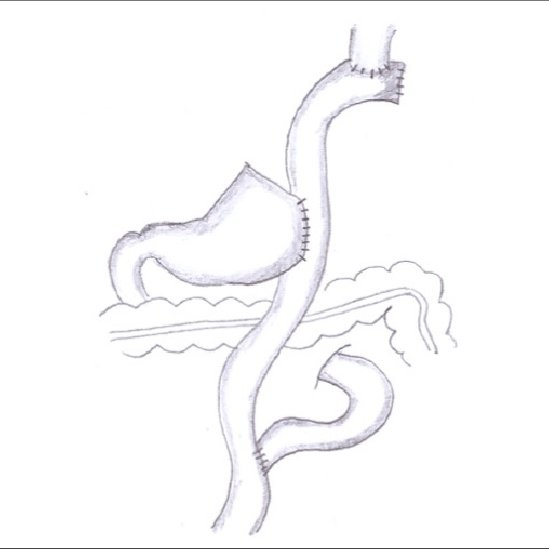
\includegraphics[width=0.5\textwidth,height=0.5\textheight]{images/Double-tract_Q640.jpg}
\caption{half-size image}\label{id}
\end{figure}

\chapter{Gastric GIST}\label{gastric-gist}

From NCCN Guidelines

\section{Genetics}\label{genetics}

\begin{itemize}
\tightlist
\item
  Mutation of KIT receptor tyrosine kinase in 80\%

  \begin{itemize}
  \tightlist
  \item
    KIT exon 9 mutations have lower response rate to imatinib and shorter progression-free survival than exon 11 mutations (especially at dose of 400mg daily)
  \end{itemize}
\item
  Mutation in PDGRFA receptor tyrosine kinase in 5-10\%. Most mutations respond to imatinib except D842V (which may respond to avapritinib)
\item
  No mutation of KIT or PDGFRA in 10-15\%. Most will have functional inactivation of SDH complex and evidenced by lack of SDHB on IHC. These patients should be tested for germline SDH mutations. These tumors tend to occur in the stomach in younger patients.
\end{itemize}

Tyrosine kinase inhibitors:

\begin{itemize}
\tightlist
\item
  imatinib - first line therapy
\item
  Sunitinib treatment is indicated for patients with imatinib-resistant tumors or imatinib intolerance.
\item
  Regorafenib is indicated for patients with disease progression on imatinib or sunitinib.
\item
  Ripretinib is indicated for patients who have received prior treatment with 3 or more kinase inhibitors, including imatinib.
\end{itemize}

\part*{Colon Cancer}\label{part-colon-cancer}
\addcontentsline{toc}{part}{Colon Cancer}

\chapter{ColonCa SCORE}\label{ColonObjCR}

\href{https://www.surgicalcore.org/modulecontent.aspx?id=1000690}{Colon Cancer SCORE}

\textbf{Physiology}

\begin{itemize}
\tightlist
\item
  APC
\item
  K-\emph{ras}
\item
  p53
\item
  microsatellite instability
\item
  CIMP
\end{itemize}

\textbf{Epidemiology}

\begin{itemize}
\tightlist
\item
  Sporadic vs hereditary vs familial
\end{itemize}

\textbf{Screening}

USPTF recommends colon cancer screening from ages 45-75

\begin{itemize}
\tightlist
\item
  Colonoscopy
\item
  Flex sig
\item
  Occult blood testing
\item
  Fecal DNA testing
\end{itemize}

\textbf{Hereditary Syndromes}

\begin{itemize}
\tightlist
\item
  Genes \textbar{} Presentation \textbar{} Screening

  \begin{itemize}
  \tightlist
  \item
    Lynch Syndrome
  \item
    APC
  \end{itemize}
\end{itemize}

\emph{Screening for average risk}

\emph{Screening for elevated risk}

\textbf{Endoscopy}

\begin{itemize}
\tightlist
\item
  Types of polyps
\end{itemize}

\textbf{Staging}

\begin{itemize}
\tightlist
\item
  CT scan
\item
  PET scan
\item
  Staging
\end{itemize}

\textbf{Adjuvant Therapy}

\begin{itemize}
\tightlist
\item
  Indications for adjuvant chemo
\end{itemize}

\textbf{Operative Treatment}

\begin{itemize}
\tightlist
\item
  Types of colectomy
\item
  Dx large bowel obstruction
\end{itemize}

\textbf{Resources}

\href{https://fascrs.org/ascrs/media/files/downloads/2022-Colon-Cancer-CPG.pdf}{ASCRS Guidelines for treatment of Colorectal Cancer 2022}

\href{https://www.uspreventiveservicestaskforce.org/uspstf/recommendation/colorectal-cancer-screening}{USPTF Colon Cancer Screening Guidelines}

\chapter{ColonCa Genetics}\label{ColonGenetics}

\textbf{Resources}

\href{https://fascrs.org/ascrs/media/files/downloads/Clinical\%20Practice\%20Guidelines/cpg_for_the_surgical_treatment_of_patients_with_lynch_syndrome_feb_2017_dcr_issue.pdf}{ASCRS Guidelines 2017}

\chapter{Partial Colectomy SCORE}\label{PColectomyObj}

\href{https://www.surgicalcore.org/modulecontent.aspx?id=129670}{Partial Colectomy CORE}

\textbf{Indications}

\textbf{Operative Anatomy}

\textbf{Preop Prep}

\begin{itemize}
\tightlist
\item
  Antibiotics
\item
  Stoma marking
\item
  Ureteral stents
\end{itemize}

\textbf{Complications}

\begin{itemize}
\tightlist
\item
  Anastomotic leak
\item
  Ureteral injury
\end{itemize}

\textbf{Resources}

\href{https://fascrs.org/ascrs/media/files/downloads/Clinical\%20Practice\%20Guidelines/clinical_practice_guidelines_for_enhanced_recovery-3.pdf}{ASCRS Guidelines for Early Recovery}

\chapter{Colostomy SCORE}\label{ColostomyObj}

\href{https://www.surgicalcore.org/modulecontent.aspx?id=1000457}{Colostomy SCORE}

\textbf{Indications}

\begin{itemize}
\tightlist
\item
  Colostomy vs Ileostomy
\end{itemize}

\textbf{Preop Prep}

\begin{itemize}
\tightlist
\item
  Stoma marking
\end{itemize}

\textbf{Operative Anatomy}

\textbf{Intraop Decision-making}

\chapter{Total Colectomy SCORE}\label{TColectomyObj}

\href{https://www.surgicalcore.org/modulecontent.aspx?id=1000583}{Total Colectomy SCORE}

\textbf{Indications}

\begin{itemize}
\tightlist
\item
  Subtotal Colectomy
\item
  Proctocolectomy
\end{itemize}

\textbf{Operative Anatomy}

\textbf{Intraop Decision-making}

\chapter{Stage I Colon Cancer}\label{stage-i-colon-cancer}

\section{Malignant colon polyp}\label{malignant-colon-polyp}

\chapter{T4 Colon Cancer}\label{t4-colon-cancer}

\section{Adjuvant HIPEC}\label{adjuvant-hipec}

COLOPEC clinlical trial \citep{klaver761}

\begin{quote}
T4 or perforated colon cancer randomized to adjuvant chemotherapy + HIPEC vs adjuvant chemotherapy alone. HIPEC with 5FU and oxliplatin. Primary endpoint was absence of peritoneal disease at laparoscopy at 18 months. 202 patients randomized. No difference in peritoneal disease-free survival at 18months. 12 (14\%) of 87 patients who received adjuvant HIPEC developed postoperative complications and one (1\%) encapsulating peritoneal sclerosis.
\end{quote}

\chapter{Stage IV Colon Cancer}\label{stage-iv-colon-cancer}

\section{Workup of Colon Cancer}\label{workup-of-colon-cancer}

CAMINO trial - Advantage of MRI over CT scan in detecting liver metastasis \citep{gorgec137}

\section{Stent vs colostomy}\label{stent-vs-colostomy}

CREST trial\citep{crestcollaborativegroup1073} stent as bridge to surgery in obstructing left colon cancers. 246 patients randomized to colostomy vs stent as bridge to surgery. Lower rate of stoma formation in stent group. Average patency of stent duration is 120 days

\section{Colon resection in stage IV colon cancer}\label{colon-resection-in-stage-iv-colon-cancer}

MSKCC: Colon surgery patients with bilobar liver metastasis treated with chemotherapy with primary tumor in place. Surgical intervention needed in 7\% of cases \citep{poultsides35}

\section{Immunotherapy for dMMR (MSI high)}\label{immunotherapy-for-dmmr-msi-high}

Colorectal cancers deficient in mismatch-repair proteins (dMMR) respond poorly to 5FU-based chemotherapy but do respond to immune-checkpoint inhibitors (\(\alpha\)-PD-1, (\(\alpha\)PD-L1, (\(\alpha\)-CTLA-4).

\href{https://www.frontiersin.org/articles/10.3389/fimmu.2022.795972/full}{Review} of immune checkpoint inhibitors in colorectal cancer

Blockade of the PD-1 (Programmed Death-1) ligand with monoclonal antibody as shows efficacy in colorectal cancer, especially those deficient in mismatch repair protein expression, as manifested by microsatellite instability (MSI-High) on pathologic exam.

Keynote-177 trial \citep{andre2207} randomized 307 patients with MSI-High dMMR colorectal cancer patients to receive either pembrolizumab or 5-FU based chemeotherapy and found superior survival with pembro.

\section{Peritoneal Colon Cancer}\label{peritoneal-colon-cancer}

\section{HIPEC}\label{hipec}

Prodige 7- Cytoreductive surgery vs cytoreductive surgery + HPIEC \citep{quenet256}

\begin{quote}
Patients with stage IV colorectal cancer randomized: 133 to the cytoreductive surgery plus HIPEC group and 132 to the cytoreductive surgery alone group. No difference in overall survival. Grade 3 or worse adverse events at 30 days were similar in frequency between groups (56 {[}42\%{]} of 133 patients in the cytoreductive surgery plus HIPEC group vs 42 {[}32\%{]} of 132 patients in the cytoreductive surgery group; p=0·083); however, at 60 days, grade 3 or worse adverse events were more common in the cytoreductive surgery plus HIPEC group (34 {[}26\%{]} of 131 vs 20 {[}15\%{]} of 130; p=0·035). Chemotherapy with oxaliplatin for 30min.
\end{quote}

CAIRO-6 Phase II Trial \citep{rovers710}

\begin{quote}
Phase II Trial of adjuvant chemotherapy Randomization to perioperative systemic therapy or CRS-HIPEC alone. Perioperative systemic therapy with CAPOX, FOLFOX, or FOLFIRI.
\end{quote}

\subsection{Peritoneal Carcinoma Index (PCI)}\label{peritoneal-carcinoma-index-pci}

Linear relationship between PCI and survival \citep{feron114}

\chapter{Colectomy}\label{colectomy-1}

\section{Extended Node dissection}\label{extended-node-dissection}

Short-term outcomes of complete mesocolic excision versus D2 dissection in patients undergoing laparoscopic colectomy for right colon cancer (RELARC): a randomised, controlled, phase 3, superiority tria

Short-term outcomes of a multicentre randomized clinical trial comparing D2 versus D3 lymph node dissection for colonic cancer (COLD trial).
Karachun A, Panaiotti L, Chernikovskiy I, Achkasov S, Gevorkyan Y, Savanovich N, Sharygin G, Markushin L, Sushkov O, Aleshin D, Shakhmatov D, Nazarov I, Muratov I, Maynovskaya O, Olkina A, Lankov T, Ovchinnikova T, Kharagezov D, Kaymakchi D, Milakin A, Petrov A.
Br J Surg. 2020 Apr;107(5):499-508. doi: 10.1002/bjs.11387. Epub 2019 Dec 24.
PMID: 31872869 Clinical Trial.

\chapter{Chemotherapy}\label{chemotherapy}

\section{Neoadjuvant Chemotherapy}\label{neoadjuvant-chemotherapy}

Seymour MT, Morton D. FOxTROT: an international randomized controlled trial in 1052 patients (pts) evaluating neoadjuvant chemotherapy (NAC) for colon cancer. J Clin Oncol. 2019 May;37(15 Suppl):3504-3504.

\chapter{Appendiceal}\label{appendiceal}

\section{Mucinous Lesions}\label{mucinous-lesions}

\href{https://www.uptodate.com/contents/appendiceal-mucinous-lesions}{Up to Date - Appendiceal Mucinous Neoplasms}

\section{Categories:}\label{categories}

\begin{itemize}
\tightlist
\item
  Low grade mucinous neoplasm - Epithelial cells with dysplasia which make mucin. LMN cells are non-invasive yet have implanted within the peritoneum (similar to endometriosis).
\end{itemize}

Mucocele - Non-ruptured LAMIN

Well-differentiated mucinous adenocarcinoma. Treatment is controversial. Neoadjuvant chemotherapy vs HIPEC.

Poorly-differentiated adenocarcinoma

\part*{Rectal Cancer}\label{part-rectal-cancer}
\addcontentsline{toc}{part}{Rectal Cancer}

\chapter{RectalCa SCORE}\label{rectalca-score}

\href{https://www.surgicalcore.org/modulecontent.aspx?id=130244}{Rectal CA SCORE}

\section{Anatomy}\label{anatomy}

-Venous drainge

\section{Presentation}\label{presentation}

\begin{itemize}
\tightlist
\item
  Assessment of sphincter function
\end{itemize}

\section{Operative Tx}\label{operative-tx}

\subsection{\texorpdfstring{\href{767-rectal_surgery.html}{Total mesorectal excision}}{Total mesorectal excision}}\label{total-mesorectal-excision}

\subsection{Transanal excision}\label{transanal-excision}

\subsection{Isolated liver mets}\label{isolated-liver-mets}

\section{\texorpdfstring{\href{770-rectal_RT.html}{Adjuvant therapy}}{Adjuvant therapy}}\label{adjuvant-therapy}

\begin{itemize}
\tightlist
\item
  Standard course chemoRT
\item
  Swedish preop RT
\item
  Total Neoadjuvant Therapy
\end{itemize}

\chapter{Objectives - APR/Exent}\label{objectives---aprexent}

\href{https://www.surgicalcore.org/modulecontent.aspx?id=162148}{APR/Exent SCORE}

\section{Indications}\label{indications-1}

-Contraindications

\section{Operative Anatomy}\label{operative-anatomy}

\section{Preop Prep}\label{preop-prep}

\begin{itemize}
\tightlist
\item
  Genetics consultation
\item
  Neoadjuvant therapy
\end{itemize}

\section{Key Steps}\label{key-steps}

\section{Intraop Decisions}\label{intraop-decisions}

\begin{itemize}
\tightlist
\item
  Intraop radiation
\item
  Vascular reconstruction
\item
  VRAM flap
\end{itemize}

\section{Complications}\label{complications}

\begin{itemize}
\tightlist
\item
  Surgical site infection
\item
  Missed enterotomy
\item
  Perineal wound dehiscence
\item
  Abdominal wound dehiscence
\item
  Urethral injury
\item
  Beeding
\item
  Ostomy necrosis
\end{itemize}

\chapter{Rectal Cancer Staging}\label{rectal-cancer-staging}

\section{MRI staging}\label{mri-staging}

Rectal cancer is preferentially evaluated with MRI. At Atrium, this is ordered as ``MRI Pelvis without Contrast Rectal Protocol''

Key findings

\begin{itemize}
\tightlist
\item
  Circumferential resection margin
\item
  Extra mesorectal vascular invasion
\item
  Mesorectal lymph nodes
\item
  Extra-mesorectal lymph nodes
\end{itemize}

MRI has supplanted endoscopic ultrasound (EUS) as the study of choice for staging rectal cancer.

MERCURY group trial demonstrated the predictive value of MRI for rectal cancer\citep{taylor34} \citep{mercurystudygroup779}

\section{EUS}\label{eus}

Endoscopic ultrasound has now been replaced by MRI for initial staging, in part due to intraoperater variability

\chapter{Rectal Ca Surgery}\label{rectal-ca-surgery}

Importance of total mesorectal excision was championed by Bill Heald \citep{heald1479} who emphasized sharp dissection of the mesorecum outside of the visceral fasial envelope. In addition he advocated dissection of the totality of the mesorectum distal to the tumor to avoid leaving behind nodes within the mesorectum distal to the tumor\citep{quirke996} \citep{nagtegaal303} \citep{paty365}.

\chapter{Rectal Adjuvant Therapy}\label{rectal-adjuvant-therapy}

\section{\texorpdfstring{Surgery \(\Rightarrow\) CRT}{Surgery \textbackslash Rightarrow CRT}}\label{surgery-rightarrow-crt}

The original approach to adjuvant therapy for rectal cancer was surgery followed by chemoradiation.

\section{\texorpdfstring{CRT \(\Rightarrow\) Surgery}{CRT \textbackslash Rightarrow Surgery}}\label{crt-rightarrow-surgery}

The next innovation to adjuvant therapy for rectal cancer was chemoradiation prior to surgery, followed by adjuvant chemotherapy.

German Rectal Cancer Study (AIO-94) compared preop and postop chemoradiation in locally-advanced rectal cancer \citep{sauer173}. Among 823 patients, local recurrence was 6\% in the preoperative group vs 13\% in the postop group (p=0.0006). Overall survival was not different, but preop chemoradiation was less toxic. Pathologic complete response rate in the preoperative group as 8\%.

NSABP R-03 clinical trial \citep{roh5124} randomized 267 patients with T3 or T4 or node-positive rectal cancer to preop vs postop chemoradiation. Disease-free survival was better in the preoperative group, wiht no difference in overall survival. Pathologic complete response rate in the preop group was 15\%. The trial did not meets its accrual targets.

Dutch Rectal Cancer Trial (CKVO 95-04): Demonstrated the benefit of preop radiation in combination with TME\citep{kapiteijn638}. Radiation reduced local recurrence form 10.9\% to 5.6\%

The Dutch trial found a reduction in local recurrence form 10.9\% to 5.6\% with preoperative radiation with no difference in survival\citep{kapiteijn638}. A later update\citep{vangijn575}

The Medical Research Council C07 trial compared preoperative short-course radiation with selective post-operative chemoradiation and found no difference in local recurrence (4.4\% vs 10.6\%) and no difference in overall survival.\citep{sebag-montefiore811}

\section{Short-course RT}\label{short-course-rt}

An alternative to preoperative chemoradiation over 6 weeks is to administer radiation alone properative over a five day period.

Swedish Rectal Cancer Trial compared surgery alone with preoperative short-course therapy consisting of 5 doses of 500cGy of radiation without chemotherapy administered in one week prior to surgery. Local recurrence was 9\% in the therapy group vs 26\% in the control group, with an improvement in overall survival of 38\% vs 80\%\citep{swedishrectalcancertrial980}. Of note, this trial was performed in the era prioro to the widespread use of total mesorectal excision.

Stockholm III trial showed that short-course radiation therapy performed 4-8 weeks prior to surgery resulted in imporved rates of pathologic complete response (12\% vs 2\%) compared with short-course radiation therapy performed the week prior to surgery \citep{pettersson972}

\section{Total Neoadjuvant}\label{total-neoadjuvant}

A more modern approach has been to administer chemotherapy in addition to chemoradiation prior to surgery, Total Neoadjuvant Therapy (TNT)

RAPIDO trial randomized 920 patients with T4 or node-positive disease to long-course chemoradiation followed by surgery vs short-course radiation followed by chemotherapy and surgery. The pCR rate was significantly higher in the short course/chemotherapy/surgery group (28\% vs 14\%) and disease-specific surival at 3years was higher (30\% vs 24\%).\citep{bahadoer29} \citep{vandervalk75}

PRODIGE 23 randomized 461 patients with T3 or T4 recta cancers to long-course radiation followed by surgery vs induction chemotherapy, long-course radiation followed by surgery. Up-front chemotherapy was associates with increased 3-year survival (76\% vs 69\%) and an increase in rate of pathologic complete response of 28\% vs 12\%.\citep{conroy702}

STELLAR trial \citep{jin1681} TNT with short-course radiation (5Gy x 5 days) + CAPEOX chemotherapy vs long-course chemoRT with capecitibine. No differences in relapse-free survival or metastasis free survival. Overall survival better with TNT (p=0.03). On subgroup analysis, no group appeared to have more benefit. pCR rate 17\% with TNT vs 13.9\% with conventional chemoradiation. Positive margins (R1) occurred in 8.5\% of TNT patients vs 12.5\% in the conventional chemoRT group.

OPRA clinical trial \citep{garcia-aguilar2546}. 324 rectal cancer patients staged with MRI randomized to INCT (induction chemo followed by chemoRT) vs CNCT (Chemoradiation followed by chemotherapy). Patients with a response were offered watch and wait. Patients without a response were treated with surgery. No difference in disease-free survival or overall survival or metastasis-free survival. 304 patients were restaged and only 26\% were recommended to have surgery. Among 225 patients in watch and wait, somewhat more patients with INCT had recurrences (40\% of 105 = 42 patients vs 27\% of 102 =32 patients). More organ preservation at 3 years with CNCT (60\% CNCT vs 47\% INCT).See also \citep{smith767}

\section{Selective Adjuvant}\label{selective-adjuvant}

Selective adjuvant therapy approaches reserves adjuvant therapy for high-risk patients, and treats low-risk patients with surgery alone.

MERCURY study group has examined selective approaches to adjuvant chemoradiation in low-risk patients with rectal cancer. \citep{taylor711}, \citep{strassburg2790}

German OCUM group \citep{kreis25} \citep{ruppert1519}

Canadian {[}Quicksilver Trial{]} (\url{https://jamanetwork.com/journals/jamaoncology/fullarticle/2730134})

\section{Neoadjuvant ImmunoTx}\label{neoadjuvant-immunotx}

Mismatch repair protein deficient (MSI-high) colorectal cancer (due to either Lynch Syndrome or BRAF-1 mutation) responds pooly to chemotherapy but responds well to immunotherapy with PD-L1 blockade

MSKCC trial of neoadjuvant PD-L1 blockade with 6 months of dostarlimab for 12 patients with MMR-deficient (MSI-high) rectal cancer resulted in 100\% clinical response rate \citep{cercek2363}. No patients were subsequently treated with either chemoradiation or surgery as originally planned.

PICC trial \citep{hu38} Chinese trial of PD-L1 blockade with neoadjvant toripalimab + colecoxib vs toripalimab for 3 months in 34 patients with MMR-deficient locally-advanced (T3/4 or N+) colorectal cancer. All patients were then treated with surgery. Pathologic complete response in 88\% of dual-therapy patients and 65\% of monotherapy. Grade 3 toxicity in 1/34 patients. Previous neoadjuvant chemo in 25\%. Rectal cancer in 18\%.

NICHE trial \citep{chalabi1949} 115 patients with dMMR locally-advanced colon cancer treated with a neoadjuvant immunotherapy. Pathologic complete response in 68\%. No recurrences with a median followo up of 26 months.

\chapter{Neoadjuvant Chemotherapy}\label{neoadjuvant-chemotherapy-1}

The PROSPECT clinical trial \citep{schrag322} randomized patients with T2/3 recctal cancer to neoadjuvant therapy with chemoradiation vs FOLFOX. 585 in the FOLFOX group and 543 in the chemoradiotherapy group. FOLFOX was noninferior to chemoradiotherapy for disease-free survival and the groups were similar with respect to overall survival. In the FOLFOX group, 53 patients (9.1\%) received preoperative chemoradiotherapy (if the primary tumor decreased in size by \textless20\% or if FOLFOX was discontinued because of side effects) and 8 (1.4\%) received postoperative chemoradiotherapy.

\chapter{Non-operative management of Rectal Cancer}\label{non-operative-management-of-rectal-cancer}

MSKCC published an experience of 113 patients with cCR after chemoradiation for rectal cancer who elected non-operative management \citep{smithe185896}. Among this group, 22 developed a local recurrence, and 8\% developed metastatic disease.\citep{smith657}

A new paradigm for rectal cancer: Organ preservation
Introducing the International Watch \& Wait Database (IWWD) \citep{beets1562}

\begin{verbatim}
Habr-Gama A.
Gama-Rodrigues J.
Sao Juliao G.P.
et al.
\end{verbatim}

Local recurrence after complete clinical response and watch and wait in rectal cancer after neoadjuvant chemoradiation: impact of salvage therapy on local disease control.
Int J Radiat Oncol Biol Phys. Mar 15 2014; 88: 822-828
View in Article

\begin{verbatim}
Maas M.
Beets-Tan R.G.
Lambregts D.M.
et al.
\end{verbatim}

Wait-and-see policy for clinical complete responders after chemoradiation for rectal cancer.
J Clin Oncol. Dec 10 2011; 29: 4633-4640
View in Article

\begin{verbatim}
Scopus (791)
PubMed
Crossref
Google Scholar

Appelt A.L.
Ploen J.
Harling H.
et al.
\end{verbatim}

High-dose chemoradiotherapy and watchful waiting for distal rectal cancer: a prospective observational study.
Lancet Oncol. Aug 2015; 16: 919-927
View in Article

\begin{verbatim}
Scopus (392)
PubMed
Abstract
Full Text
Full Text PDF
Google Scholar

Smith J.D.
Ruby J.A.
Goodman K.A.
et al.
\end{verbatim}

Surveillance after neoadjuvant therapy in advanced rectal cancer with complete clinical response can have comparable outcomes to total mesorectal excision.
Int J Colorectal Dis. Jun 2015; 30: 769-774

\chapter{Anal Squamous Cell Carcinoma}\label{anal-squamous-cell-carcinoma}

\href{https://www.nccn.org/professionals/physician_gls/pdf/anal_blocks.pdf}{NCCN Guidelines}

Surgical Clinics Review Article: \citep{young629}

\section{Chemoradiation}\label{chemoradiation}

Chemoradiation is now the standard for anal squamous cell carcinoma of the anal canal and for perianal cancers (except for small T1 lesions). Nigro protocol is the standard approach.\citep{nigro1826}

\subsection{Restaging after chemoRT}\label{restaging-after-chemort}

Based on the results of the ACT-II study, it may be appropriate to follow patients who have not achieved a complete clinical response with persistent anal cancer up to 6 months following completion of radiation therapy and chemotherapy as long as there is no evidence of progressive disease during this period of follow-up. Persistent disease may continue to regress even at 26 weeks from the start of treatment.\citep{james516}

\part*{Sarcoma}\label{part-sarcoma}
\addcontentsline{toc}{part}{Sarcoma}

\chapter{Soft Tissue Sarcomas}\label{soft-tissue-sarcomas}

\section{Desmoid Tumors}\label{desmoid-tumors}

Review of desmoid tumors: \href{https://www.ejcancer.com/article/S0959-8049(19)30832-9/fulltext}{Global Consensus Guidelines}

\section{Retroperitoneal}\label{retroperitoneal}

\textbf{Preop Radiation}

STRASS trial randomized 266 patients to preop radiation followed by surgical resection vs surgery alone. At a median followup of 43 months, there was no difference in recurrence-free survival. Serious adverse affects were more common in the preop radiation group (24\% vs 10\%). One patients in the radiation group died of treatment-related toxicity (gastrocolic fistula), compared with none in the surgery alone group \citep{bonvalot1366}. See commentary: \citep{cardona1257}

STRASS2: Ongoing trial of neoadjuvant chemotherapy.

\section{Peritoneal mesothelioma}\label{peritoneal-mesothelioma}

Review \citep{bridda32}

Surgical Oncology Clinics review \citep{li539}

\part*{Small Bowel}\label{part-small-bowel}
\addcontentsline{toc}{part}{Small Bowel}

\chapter{Small Bowel Neoplasms}\label{small-bowel-neoplasms}

\section{Carcinoid}\label{carcinoid}

\section{Adenocarcinoma}\label{adenocarcinoma}

  \bibliography{zotero.bib}

\end{document}
